% !TEX encoding = UTF-8 Unicode

% Format teze zasnovan je na paketu memoir
% http://tug.ctan.org/macros/latex/contrib/memoir/memman.pdf ili
% http://texdoc.net/texmf-dist/doc/latex/memoir/memman.pdf
% 
% Prilikom zadavanja klase memoir, navedenim opcijama se podešava 
% veličina slova (12pt) i jednostrano štampanje (oneside).
% Ove parametre možete menjati samo ako pravite nezvanične verzije
% mastera za privatnu upotrebu (na primer, u b5 varijanti ima smisla 
% smanjiti 
\documentclass[12pt,oneside]{memoir} 

% Paket koji definiše sve specifičnosti master rada Matematičkog fakulteta
\usepackage[latinica,biblatex]{matfmaster} 

\usepackage{amsmath}
% \usepackage{color}
% \usepackage{url}
% \usepackage[utf8]{inputenc} % make weird characters work
\usepackage{graphicx}
\graphicspath{{figures/}} %Setting the graphicspath

% \usepackage[english,serbian]{babel}
% \usepackage[english,serbianc]{babel} %ukljuciti babel sa ovim opcijama, umesto gornjim, ukoliko se koristi cirilica

\usepackage[unicode]{hyperref}
\hypersetup{colorlinks,citecolor=green,filecolor=green,linkcolor=blue,urlcolor=blue}

\usepackage[figure]{algorithm}
\floatname{algorithm}{Pseudokod}
\usepackage[noend]{algpseudocode}

%header
% \usepackage{fancyhdr}
% \pagestyle{fancy}

%\newtheorem{primer}{Пример}[section] %ćirilični primer
\newtheorem{primer}{Primer}[section]
\newtheorem{defi}{Definicija}[section]
\newtheorem{teo}{Teorema}[section]

% Datoteka sa literaturom u BibTex tj. BibLaTeX/Biber formatu
\bib{master}

% Ime kandidata na srpskom jeziku (u odabranom pismu)
\autor{Nikola Dimitrijević}
% Naslov teze na srpskom jeziku (u odabranom pismu)
\naslov{Algoritmi za otkrivanje kolizije u realnom vremenu}
% Godina u kojoj je teza predana komisiji
\godina{2019}
% Ime i afilijacija mentora (u odabranom pismu)
\mentor{doc. dr Vesna \textsc{Marinković} \\ Univerzitet u Beogradu, Matematički fakultet}
% Ime i afilijacija prvog člana komisije (u odabranom pismu)
\komisijaA{prof. dr Predrag \textsc{Janičić } \\ Univerzitet u Beogradu, Matematički fakultet}
% Ime i afilijacija drugog člana komisije (u odabranom pismu)
\komisijaB{dr Ivan \textsc{Čukić} \\ Univerzitet u Beogradu, Matematički fakultet}
% Datum odbrane (odkomentarisati narednu liniju i upisati datum odbrane ako je poznat)
\datumodbrane{ }

% Apstrakt na srpskom jeziku (u odabranom pismu)
\apstr{%
 Rezime.
}
 
% Ključne reči na srpskom jeziku (u odabranom pismu)
\kljucnereci{detekcija kolizije, računarska grafika, vremenska koherentnost, algoritmi}

\begin{document}
% ==============================================================================
% Uvodni deo teze
\frontmatter
% ==============================================================================

% Naslovna strana
\naslovna
% Strana sa podacima o mentoru i članovima komisije
\komisija
% Strana sa posvetom (u odabranom pismu)
% \posveta{Mami, tati i dedi}
% Strana sa podacima o disertaciji na srpskom jeziku
% \apstrakt
% Sadržaj teze
% \pagenumbering{arabic}

\begingroup
\vspace*{-5\baselineskip}
\tableofcontents
\endgroup

\mainmatter

% ==============================================================================
\chapter{Uvod}
\label{sec:uvod}
% ==============================================================================

Problem detekcije kolizije ima naizgled veoma jednostavan zadatak: naći sve parove objekata
koji se presecaju. Pored parova objekata, nekada je potrebno odrediti i oblik preseka
ili precizan trenutak u kome objekti počinju da se presecaju. 
Realizacija uspešnog algoritma detekcije kolizije zahteva korišćenje 
koncepata iz računarske grafike i računarske geometrije.

Nije teško konstruisati naivni algoritam koji utvrđuje da li postoji presek jednostavnih geometrijskih tela.
Međutim, današnji virtuelni svetovi sadrže hiljade pokretnih tela i stotine miliona poligona i 
zato je potrebno koristiti napredne strukture podataka i razviti efikasne algoritme. 
Nedovoljno efikasan algoritam za otkrivanje kolizije može predstavljati usko grlo sistema.

Objekat čiji se presek razmatra može biti jednostavan kao što je kocka, a može biti izgrađen i od desetine hiljada poligona.
Stoga nije praktično da se za svaki poligon svakog od razmatranih objekata
proverava da li postoji presek sa nekim poligonom nekog drugog objekta.
Umesto toga, složeni objekti se zamenjuju kvadrima koji su opisani oko njih.
Na taj način se najpre razmatraju jednostavniji objekti, pa tek ako se oni seku ispituje se da li postoji presek konkretnih poligona od kojih je objekat sastavljen.
%
Prvi deo ovog postupka naziva se \textbf{široka faza} (eng. {\em broadphase}), a drugi deo se naziva \textbf{uska faza} (eng. {\em narrowphase}).
Drugi deo ovog procesa nije uvek neophodan, na primer kada su svi objekti čiji se presek razmatra kocke, kao što je to slučaj u nekim igrama.
Ovaj rad je usmeren na široku fazu pošto je ona od ključnog značaja kada se radi o velikom broju objekata.
Razlog za to je taj što je problem koji ona rešava u najgorem slučaju kvadratne vremenske i prostorne složenosti
jer je broj parova objekata koji se presecaju u najgorem slučaju $O(n^2)$, 
gde je $n$ broj objekata koji se razmatra.
Uglavnom je broj parova objekata koji se presecaju neznatan u odnosu na broj potencijalnih parova. 
Zato je uticaj uske faze na performanse manji u odnosu na široku fazu za koju je važno imati što efikasniju implementaciju.

Za interaktivne svetove je neophodno otkrivanje kolizija u realnom vremenu. 
Potreba izvršavanja u realnom vremenu nosi sa sobom nove probleme za čije rešavanje se koriste posebni mehanizmi 
i uglavnom dolazi do kompromisa između preciznosti detekcije kolizije i efikasnosti algoritama.

U prvom poglavlju rada biće data motivacija. 
Pregled relevantnih pojmova i fenomena biće prikazanu u drugom poglavlju uz fokus na konzistentne korake izvršavanja.
Algoritmi široke faze biće predstavljeni u trećoj glavi. 
Implementacija projekta biće opisana u četvrtoj, 
a evaluacija performansi i demonstracija nekih principa biće razmotrena u petoj glavi.
U poslednjoj glavi biće dati glavni zaključci ovog rada i mogući pravci za dalji rad.

\section{Motivacija}
\label{sec:naslov1}
Otkrivanje kolizije ima široke primene u kontekstu virtuelne realnosti, računarskih igrara, planiranja putanje robota,
dizajna uz pomoć računara (eng. {\em Computer aided design, CAD}) i fizičkih simulacija. 
Za neke od navedenih primena zahtev realnog vremena nije neophodan, na primer za planiranje putanje robota ili renderovanje računarski generisanih slika filmova.
Međutim, detekcija kolizije u realnom vremenu predstavlja ključni deo svakog pogona igre (eng. {\em game engine}), a danas ga svaka složenija
video igra koristi. Industrija video igara svake godine raste \cite{game_industry}
u toj meri da ima veći prihod od filmske i muzičke industrije zajedno! Zaista, 2018. godine industrija igara imala je prihod od
137 milijardi američkih dolara naspram 41 milijarde filmske i 17 milijardi dolara prihoda muzičke industrije \cite{movie, music, game_industry}.
Posledice manjih grešaka (bagova) u igrama nisu dramatične poput potencijalnih posledica neispravnog softvera u avionskoj ili automobilskoj industriji, ali 
se svakako negativno odražavaju na prihod.
Korisnici očekuju visok stepen doteranosti video igara, pa bi postojanje velikog broja bagova 
obeshrabrilo potencijalne kupce. Na slici \ref{fig:batman} je prikazana greška gde igrač propada kroz
pod virtuelnog sveta, a na slici \ref{fig:horse} igrač ne može da se popne na konja pošto on lebdi u vazduhu.

Na tržištu se poslednjih godina pojavljuju rukavice za virtuelnu realnost koje simuliraju dodir virtuelnih objekata, a za njih je 
detekcija kolizije i izvršavanje u realnom vremenu od presudnog značaja.
Potrebno je bar 1000 puta u sekundi pružiti povratnu informaciju korisniku da bi simulacija dodira bila uverljiva \cite{haptic}. 

\begin{figure}
\centering
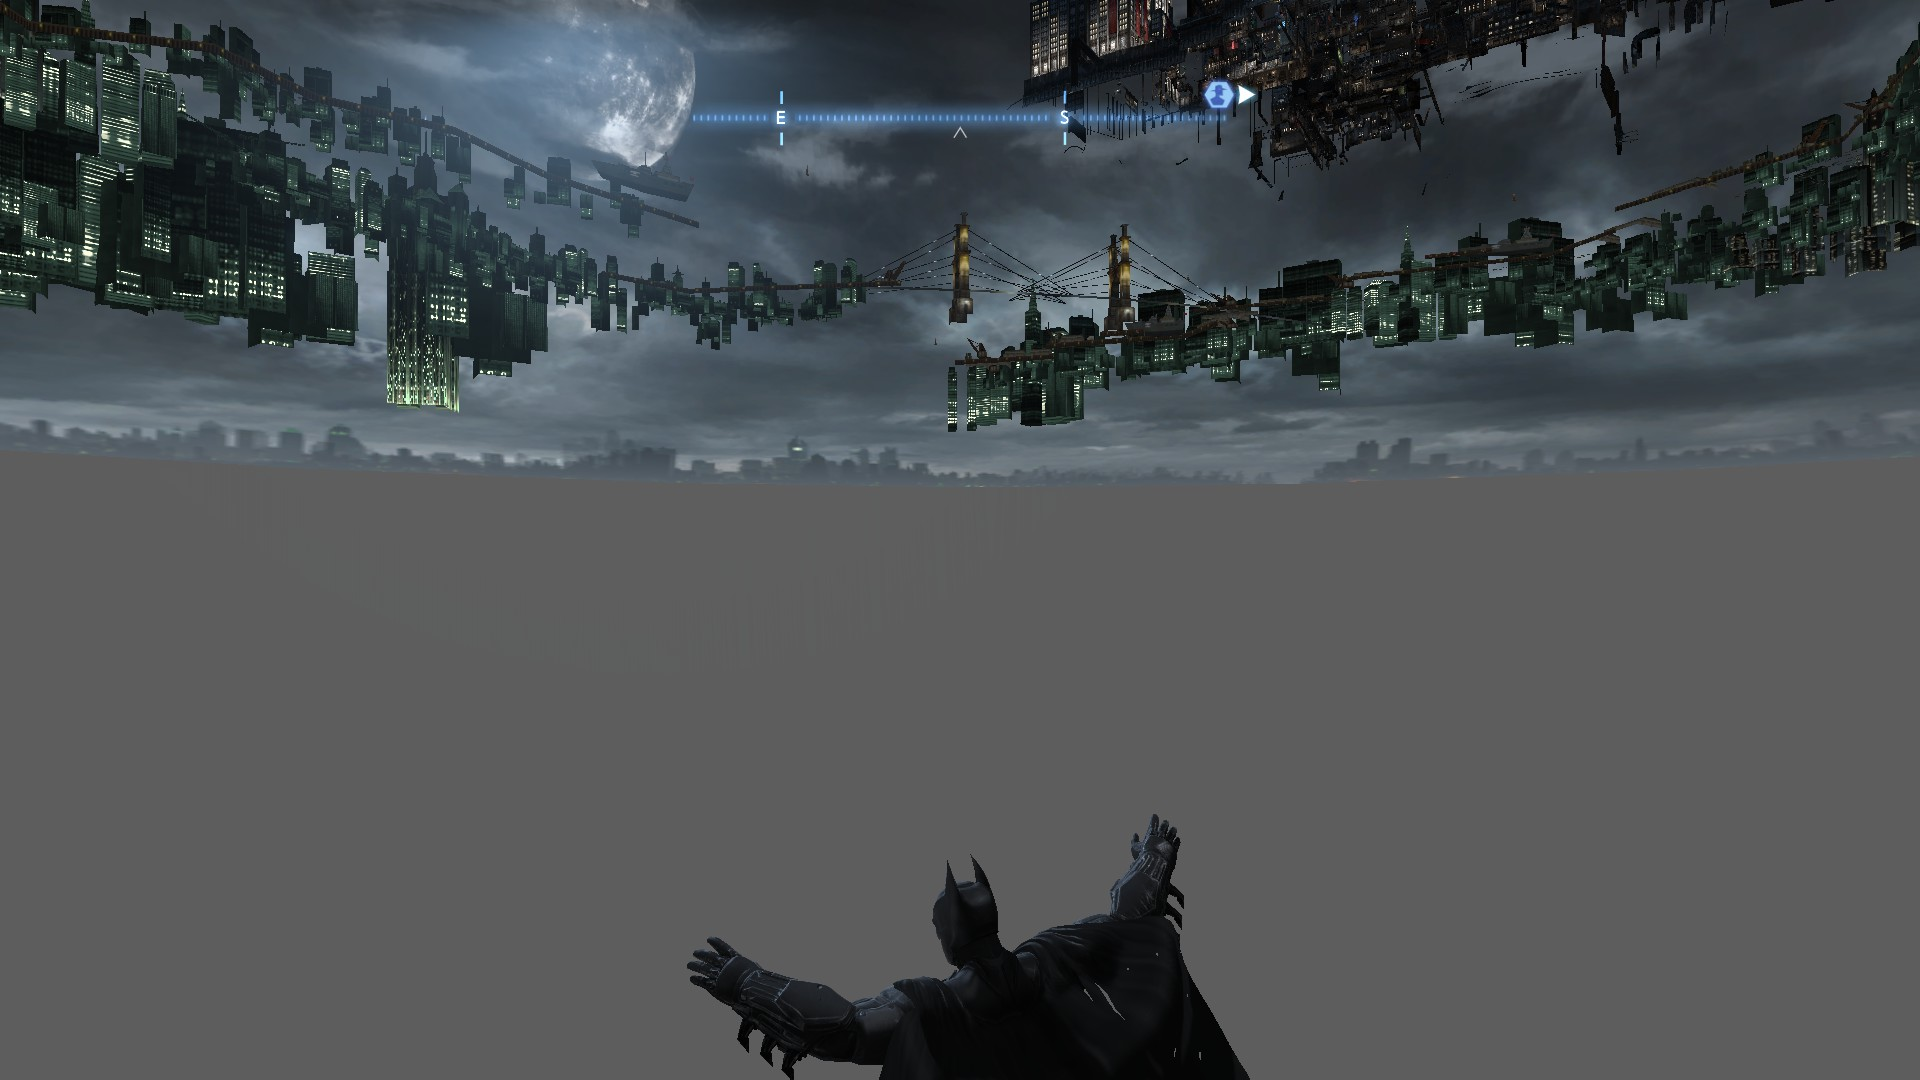
\includegraphics[scale=0.22]{batman.jpg}
\caption{Propadanje ispod modelovanog sveta (\tiny preuzeto sa \url{ https://tinyurl.com/y5g987j5 }).}
\label{fig:batman}
\end{figure}


\begin{figure}
	\centering
	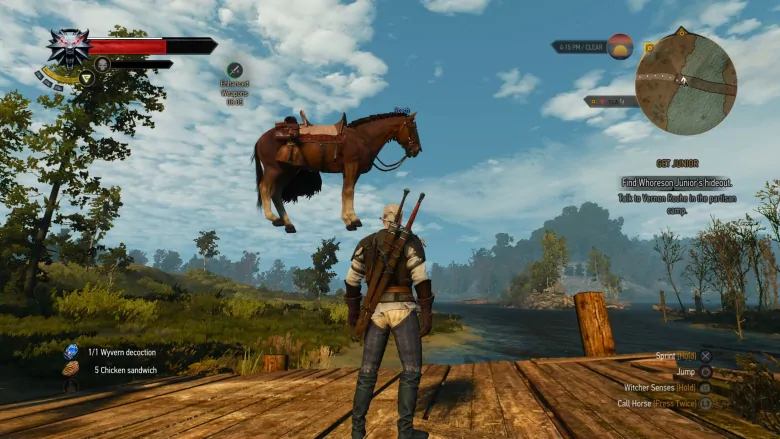
\includegraphics[scale=0.54]{horse.png}
	\caption{Levitirajući konj (\tiny preuzeto sa \url{ https://tinyurl.com/y6qbaxqm }).}
	
	\label{fig:horse}
\end{figure}

Problem detekcije kolizije svih parova objekata je u najgorem slučaju kvadratne vremenske i prostorne složenosti 
jer se može desiti da se svaka dva objekta seku, te je maksimalni broj parova objekata koji su u koliziji reda $O(n^2)$, 
gde je $n$ broj objekata koji se razmatra.
Međutim, broj preseka je najčešće mnogo manji od ove gornje granice.
Ipak, postoje slučajevi kada je vreme izvršavanja algoritma reda $\Theta(n^2)$, na primer u situaciji kada se svaka dva objekta seku.

Potreba da se algoritam izvršava u realnom vremenu je očigledna kod interaktivnih primena.
Međutim i za neinteraktivne primene, potrebno je imati što efikasniji algoritam za utvrđivanje kolizije koji bi mogao da se često pokreće.
Filmovi nisu interaktivan sadržaj i zato je učestalost osvežavanja slike od 24Hz, uz korišćenje zamućivanja pokreta (eng. {\em motion blur}),
dovoljno dobra za većinu ljudi. Standard za igre na konzolama je barem 30Hz, a na desktop računarima  barem 60Hz. 
Za primene u oblasti virtuelne realnosti potrebno je postići učestalost osvežavanja slike od barem 90Hz, jer manje frekvencije često prouzrokuju
dezorijentaciju, mučninu i druge neželjene efekte kod korisnika \cite{importance}.

Ne postoji najbolji algoritam za detekciju kolizije koji će pokriti svaki mogući slučaj. 
Neki algoritmi su dobri za uniformno raspoređene objekte u prostoru, ali pokazuju loše performanse kada su svi objekti na jednom mestu, 
dok na druge algoritme manje utiče prostorni raspored objekata ali im efikasnost varira u zavisnosti od brzine kretanja objekata.
Takođe, isti algoritam može imati značajno bolje performanse ako su njegovi parametri dobro 
izabrani za neku hardversku arhitekturu ili za očekivani raspored objekata. 
Sve pomenute činjenice inspirisale su razvoj aplikacije koja omogućava brzo i interaktivno menjanje
algoritama detekcije kolizije, postavljanje njihovih parametara kao 
i  posmatranje performansi trenutno odabranog algoritma za dati izbor parametara.

% ==============================================================================
\chapter{Pregled relevantnih pojmova}
\label{sec:karakteristike}
% ==============================================================================

U ovom poglavlju biće opisani mehanizmi i fenomeni čije je poznavanje potrebno za razumevanje i konstrukciju 
efikasnog rešenja problema detekcije kolizije.
Algoritam detekcije kolizije se ne koristi kao izolovani algoritam nego se izvršava paralelno sa renderovanjem slike,
puštanjem zvuka, mrežnom komunikacijom, rukovanjem ulaza, animacijama, simulacijom fizike, itd. 
Zato treba uzeti u obzir sve relevantne činjenice koje utiču na performanse implementacije.

\section{Faze problema detekcije kolizije}

Celokupan zadatak detekcije kolizije se deli na dve faze: široku fazu i usku fazu. 
U prvoj, širokoj fazi
odbacuje se (često) većina kandidata od svih mogućih parova objekata za koje se ispituje da li se seku.
Cilj pri implementaciji široke faze je razviti što efikasniji algoritam (u funkciji broja objekata) 
za pronalaženje parova objekata koji se eventualno mogu seći.
Zadatak uske faze je da se za parove objekata dobijenih u širokoj fazi utvrdi da li oni zaista imaju presek.
Iako postoje takvi slučajevi, u mnogim primenama nisu svi objekti prosta geometrijska tela poput kocki, kvadara ili lopti.
Objekti koji se razmatraju mogu biti veoma složeni, predstavljeni u vidu kompozicije velikog broja prostijih tela ili kao mreže sastavljene od stotina hiljada trouglova.
U ovim situacijama veoma je važno osmisliti i razmatrati nekakvu jednostavniju reprezentaciju tih objekata.

\textbf{Granični opsezi} (eng. {\em bounding volume}) prestavljaju jedan tip jednostavnije reprezentacije \cite{rgpdf}.
Za granične opsege se uglavnom koriste kvadri, a pored toga se mogu koristiti sfere, kapsule i druga tela.
Ono što se najčešće radi jeste da se naprave najmanje "kutije" koje će sadržati u potpunosti te objekte.
Te "kutije" su u obliku kvadra čije su strane poravnate sa osama koordinatnog sistema i nazivaju se
\textbf{ograničavajuće kutije poravnate prema osama} (eng. {\em Axis Aligned Bounding Box}), skraćeno \textbf{AABB}.
Umesto da se računaju preseci između velikog broja prostih objekata od kojih su tela sastavljena, sada se posmatraju 
samo preseci među kutijama. tj. uprošćenim reprezentacijama tela.

Umesto AABB moguće je koristiti konveksne omotače tela ili \textbf{orijentisane ograničavajuće kutije} (eng. {\em Oriented Bounding Box}), skraćeno \textbf{OBB}.
Orijentisane ograničavajuće kutije su kvadri čije strane ne moraju biti paralelne baznim osama, 
već se mogu slobodno rotirati (orijentisati) tako da uže opišu telo koje reprezentuju.
\textbf{Hijerarhije graničnih opsega} (eng. {\em Bounding Volume Hierarchy}), skraćeno \textbf{BVH}, su stabla koja se grade rekurzivnom podelom 
prostora na granične opsege. Što je granični opseg bliže telima koje aproksimira to bolje, pošto to vodi do manjeg broja 
lažno pozitivnih kolizija na koje se bez razloga troši vreme u uskoj fazi. 
Hijerarhije graničnih opsega mogu za granične opsege koristiti npr. AABB ili OBB.
BVH koja koristi OBB je fleksibilnija od one koja koristi AABB jer se ograničavajuće kutije slobodno rotiraju 
i tako mogu uže da opišu tela čije uprošćenje predstavljaju. 
Ipak, zbog složenije provere preseka i zbog nepoznavanja dobrih metoda konstrukcije hijerarhije graničnih
opsega, rešenje koje koristi OBB nije nikada zaživelo u praksi \cite{obb}. 

Danas se najčešće koriste stabla izgrađena od AABB poput oktrija opisanog u \ref{subsec:octree} i njegovih modifikacija. 
Teorema o razdvajajućim osama daje inspiraciju za konstrukciju algoritma provere kolizije koristeći AABB.

\begin{teo}
	\textbf{[Teorema o razdvajajućim osama]}
	\label{teo:sat}
	Dva konveksna objekta se ne presecaju ako postoji prava (osa) 
	tako da se projekcije objekata na tu pravu ne seku.
\end{teo}

Nezavisno od dimenzionalnosti, razdvajajuća osa je uvek prava. Na primer, trodimenzionalan prostor
je razdvojiv ravnima, ali razdvajajuća osa je normalna na razdvajajuću ravan.

Prema teoremi \ref{teo:sat} dovoljno je pronaći samo jednu pravu tako da se projekcije tela na njoj ne presecaju.
Moguće je, na primer, da se uzmu normale svih strana jednog triangulisanog tela, izračunaju projekcije drugog 
tela na svaku pravu, i ako za neku od tih pravih važi da ne postoji presek projekcije drugog objekta sa projekcijom strane kroz koju prolazi prava, onda se razmatrana tela ne seku.
Međutim, ovakav pristup nije dovoljno dobar za potrebe detekcije kolizije u realnom vremenu. 
Zato se  ova teorema primenjuje samo za proveru preseka između AABB.

Teorema o razdvajajućim osama je takođe korisna za pronalaženje \textbf{minimalnog vektora translacije} (eng. {\em minimum translation vector}), odnosno
vektora najmanjeg intenziteta za koji je potrebno translirati jedan objekat da bi objekti prestali da se seku.
Najčešće se simuliraju interakcije objekata koji su čvrsti i ne mogu prolaziti jedni kroz druge.
Zato je potrebno njihovo odbijanje predstaviti promenom pravca kretanja i postarati se da ti objekati više nemaju presek.
Zbog toga, kada se ustanovi da se dva objekta presecaju potrebno je translirati ih tako da oni više nemaju presek i promeniti im vektore brzina.
Taj postupak se naziva \textbf{razrešenje kolizije} (eng. {\em collision resolution}) i opisan je u delu \ref{sec:razresenje} i u njemu ključnu ulogu igra minimalan vektor translacije.

Kada se utvrdi da postoji presek između dva AABB, to ne znači da zaista postoji presek između dva objekta
sadržana u datim AABB, čak i ako su ti objekti konveksni. Jedan takav slučaj je prikazan na slici \ref{fig:2dfalse}. 

\begin{figure}[h!]
	\centering
	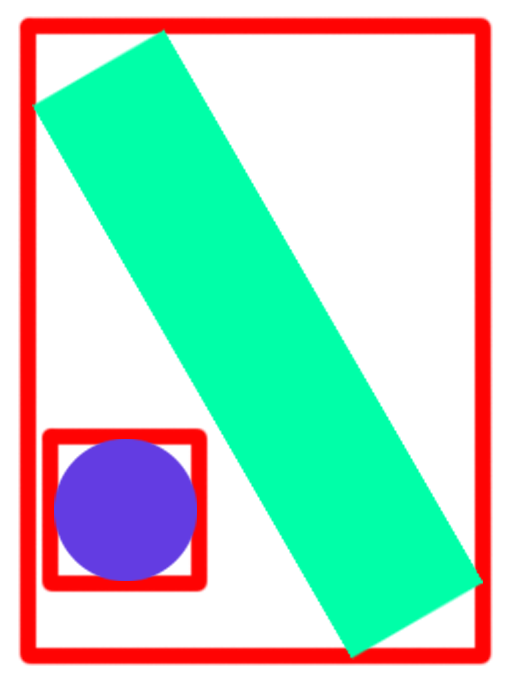
\includegraphics[scale=0.2]{2dfalseCol.png}
	\caption{Krug i rotiran pravugaonik nemaju presek dok njihovi granični opsezi imaju.}
	\label{fig:2dfalse}
\end{figure}

%https://www.scss.tcd.ie/~manzkem/CS7057/cs7057-1516-07-NarrowPhase-mm.pdf
Utvrđivanje da li postoji presek objekata sadržanih u AABB koji se seku radi se u uskoj fazi.
U slučaju kada su objekti unutar AABB neka prosta geometrijska tela poput
lopte ili kvadra može se primeniti teorema o razdvajajućim osama da bi se videlo da li zaista postoji presek među njima. 


Međutim, nije dovoljno razmatrati samo projekcije na koordinatne ose, 
jer na primeru sa slike \ref{fig:2dfalse} vidi se da se krug i rotiran pravougaonik ne presecaju, iako se njihove projekcije 
na koordinatne ose seku. Za konveksne objekte je moguće naći neku drugu pravu koja ih razdvaja ili odrediti postojanje preseka 
na neki drugi način, ali se to ostavlja za usku fazu.

% https://en.wikipedia.org/wiki/User:Oleg_Alexandrov/Pictures
\begin{figure}[h!]
	\centering
	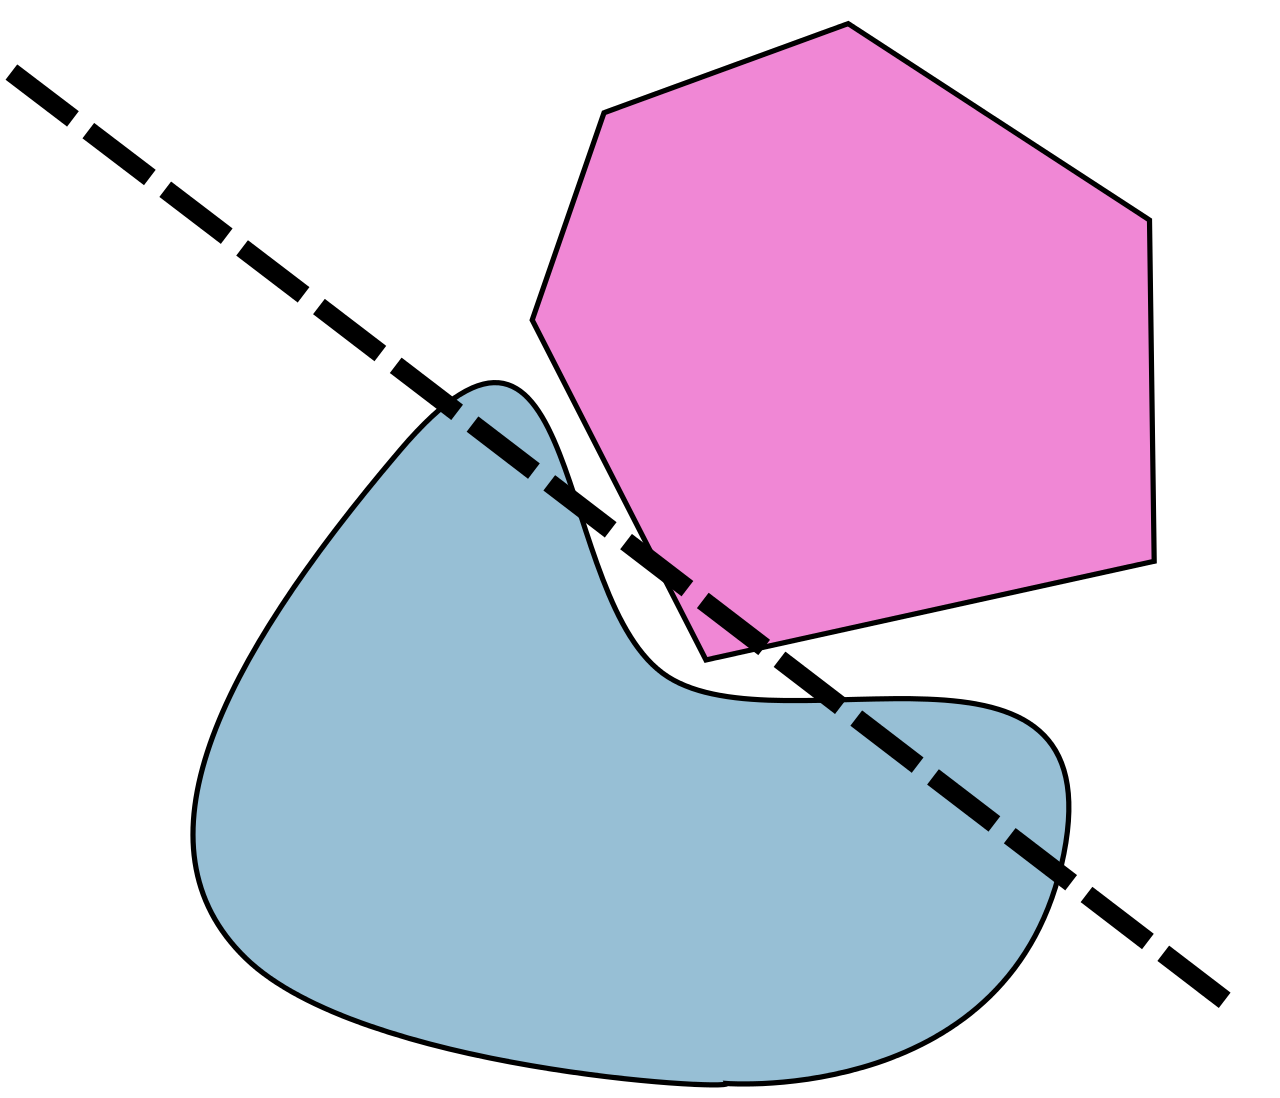
\includegraphics[scale=0.17]{theorem_counterexample.png}
	\caption{Projekcija nekonveksne površi na pravu (\tiny preuzeto sa \url{ https://tinyurl.com/yxbqg5hq }).}
	
	\label{fig:counter}
\end{figure}

Na slici \ref{fig:counter} prikazane su dve površi, jedna konveksna a druga nekonveksna. 
Za svaku pravu se projekcije datih površi na njoj seku, iako površi u stvari nemaju presek.
Dakle, teorema o razdvajajućim osama ne važi za nekonveksne objekte. 
Primer u tri dimenzije dat je na slici \ref{fig:falseCollision}, gde iako ne postoji presek dva objekta, 
tek u uskoj fazi može se zaključiti da se objekti ne seku.

\begin{figure}[h!]
	\centering
	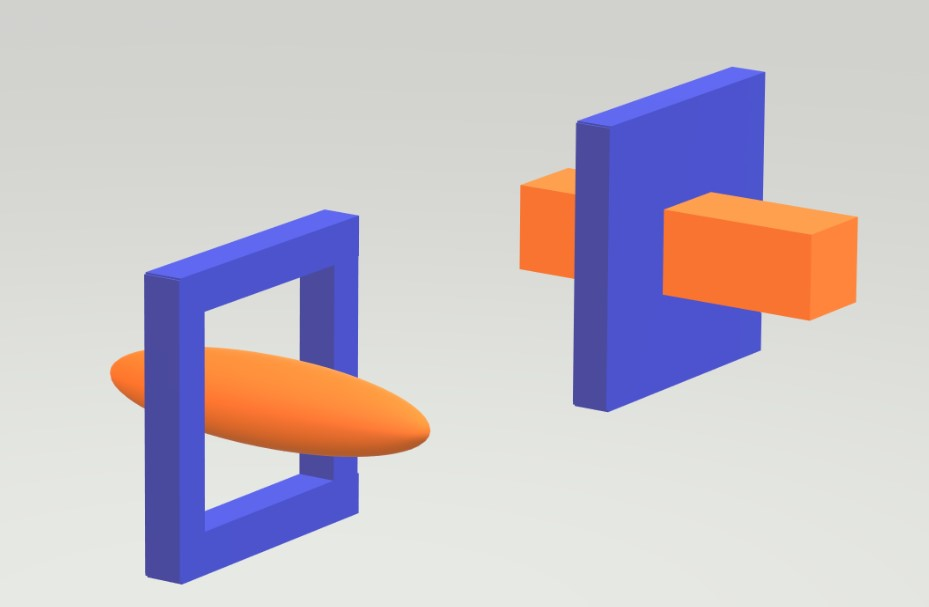
\includegraphics[scale=0.5]{falseCollision.jpg}
	\caption{Konveksan i nekonveksan objekat u prostoru bez preseka sa leve strane i
	njihovi granični opsezi koji se presecaju sa desne strane. }
	\label{fig:falseCollision}
\end{figure}


\section{Konzistentnost vremena izvršavanja}

Prilikom razmatranja vremena izvršavanja algoritma, nekada je od interesa 
samo ukupno vreme koje je potrošeno za izvršavanje većeg broja iteracija provere da li je došlo do kolizije. 
Međutim, to nije dovoljno dobro za potrebe izvršavanja algoritma u realnom vremenu.
Ako samo jedna iteracija 
detekcije kolizije traje višestruko duže od ostalih onda dolazi do takozvanog "seckanja"
koje, ukoliko se dešava često, dovodi do neupotrebljivog proizvoda.
Razmatranjem sledeće situacije se uviđa još jedan problem.

Ekrani imaju fiksnu učestalost osvežavanja slike koja najčešće iznosi 60Hz, mada postaju sve popularniji
% https://www.blurbusters.com/faq/120hz-monitors/
ekrani sa 120Hz, 144Hz, pa čak i 240Hz. Dakle ekran od 60Hz će svakih 16.67 milisekundi prikazati sledeću sliku. 
Ako se između dva osvežavanja ekrana uvek pripremi nova slika to je odlično. 
Još bolje je kada se nova slika izračunava neposredno pre osvežavanja ekrana jer se onda 
prikazuje verodostojnija slika za taj trenutak. 
Svakako će uvek postojati neko kašnjenje od trenutka interakcije korisnika sa igrom ili simulacijom do
trenutka kada se prikaže slika, ali je cilj da to kašnjenje bude što manje. 
Kada se u jednom ciklusu osvežavanja ekrana pripremi više od jedne slike, onda se uzima ona koja je najnovija,
a prethodne se odbacuju. 
Dakle praktično je protraćeno vreme uloženo u pravljenje svih slika osim poslednje.
Kada nije izračunata nova slika za sledeći ciklus osvežavanja ekrana onda će opet biti prikazana slika
iz prošlog ciklusa. Tada se gubi na glatkoći prikazanog sadržaja i na brzini odziva programa. 

Broj slika po sekundi (eng. {\em frames per second}), skraćeno \textbf{fps}, je broj slika koje program napravi u jednoj sekundi.
Naizgled ako program ima 60fps to je savršeno za ekran od 60Hz. To ipak ne mora da bude slučaj.
U toku jedne sekunde u prvih 500 milisekundi može biti kreirano 59 slika, a u preostalih 500 milisekundi samo jedna nova slika. 
To zaista jeste 60fps, ali ono što je prikazano na ekranu nije mnogo bolje od 2fps, 
što je praktično nedopustivo. 
Dakle, sa jedne strane nije dobar višak slika jer se nepotrebno troše resursi na njih iako se ne prikazuju, 
a sa druge strane manjak slika i njihovo neravnomerno generisanje dovodi do neprijatnosti.
Zato je bitno da cela simulacija, a samim tim i detekcija kolizije ima što konzistentnije vreme izvršavanja.
Konzistentno vreme izvršavanja podrazumeva da je vreme između dve prikazane slike isto.

Na slici \ref{fig:fpsdiv2} se vidi da je kreirano 6 slika, tj. da program praktično ima 6fps, iako je prikaz na ekranu 
ekvivalentan sa 3fps, što je još jedan primer nepoželjne posledice nekonzistentnog vremena izvršavanja. 

\begin{figure}[h!]
	\centering
	
\includegraphics[scale=0.5]{fpsdiv2.png}
	\caption{ Trenuci kreiranja nove slike (crvena boja) i trenuci osvežavanja ekrana (crna boja) koji su loše sinhronizovani. }
	\label{fig:fpsdiv2}
\end{figure}

\section{Vremenska koherentnost}

Često je cilj odrediti ne samo kolizije za tekuću scenu, već i kolizije u trenutku koji ubrzo sledi.
Objekti na sceni se uglavnom ne teleportuju već se postepeno kreću kako vreme teče.
Tako su pozicije objekata u bliskim trenucima slične i to se može iskoristiti za dodatno ubrzanje algoritama detekcije kolizije. 
Opšti princip je da se čuvaju svi parovi objekata koji se seku i da se u svakoj iteraciji 
izbace oni parovi objekata koji više nisu u koliziji a dodaju oni koji su od tog trenutka u koliziji.
Na taj način se značajno smanjuje vreme potrebno za izračunavanje kolizija kroz iteracije.
U slučaju da se objekti jako sporo ili uopšte ne kreću 
vremenska složenost svake iteracije algoritma biće linearna (ovo tvrđenje biće kasnije detaljnije razmatrano).


\subsection{Vremenski antialiasing}

\textbf{Vremenski aliasing} (eng. {\em temporal aliasing}) je vizuelni fenomen koji 
nastaje kada se generiše nedovoljan broj slika u sekundi u odnosu na brzinu kretanja objekata na sceni.
\textbf{Vremenski antialiasing} ima za cilj da smanji ili ukloni efekte vremenskog aliasinga.
Usled vremenskog aliasinga objekti izgledaju kao da poskakuju umesto da odaju utisak glatkog kretanja,
ili se naizgled kreću u suprotnom smeru od stvarnog.
Da bi se izbegao vremenski aliasing potrebno je da broj slika scene u sekundi bude bar duplo veći 
od brzine objekta koji se najbrže kreće \cite{Grant}. 
Jedan od često viđanih primera vremenskog aliasinga je da se na snimku točkovi automobila naizgled kreću unazad.

Vremenski antialiasing se takođe koristi za smanjenje oštrih ivica koje trepere kada se pomera kamera.
Na slici \ref{fig:txaa} se vidi jasno poboljšanje izgleda ivica kada se koristi TXAA,
tehnika koju koristi kompanija NVIDIA da bi umanjila efekat vremenskog i prostornog aliasinga.
Prostorni aliasing nastaje usled prikazivanja slike veće rezolucije na nižoj rezoluciji.
MSAA (eng. {\em multisample anti-aliasing}) je tehnika umanjenja prostornog aliasinga 
uzimanjem više uzoraka vrednosti boja u svakom pikselu.
Na slici \ref{fig:txaa} prikazan je i efekat primene MSAA, ali ta tehnika ovde nije značajna 
pošto vreme između dve generisane slike i brzina kretanja objekta ne utiču na njeno izvršavanje.

\begin{figure}[h!]
	\centering
	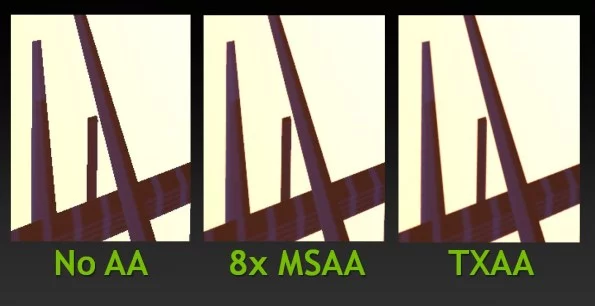
\includegraphics[scale=0.65]{txaa.png}
	\caption{Upoređivanje tehnika antialiasinga (\tiny preuzeto sa \url{ https://tinyurl.com/y2c6nw5l }).}
	
	\label{fig:txaa}
\end{figure}

\section{Preciznost i preseci zapremina pokretnih tela}

Koliziju je moguće utvrđivati sa različitim nivoom preciznosti. 
Pod preciznošću se podrazumevaju dve stvari: da li su otkrivene sve kolizije koje su se desile i 
da li se objekti koji se iscrtavaju reprezentuju uprošćeno za svrhe kolizije. 
Jasno je da veća preciznost sa sobom iziskuje veće vremenske i prostorne resurse. 
Stoga se često bira nešto nepreciznija varijanta koja ima kraće vreme izvršavanja i manju potrošnju memorije.

Pošto se provera kolizije vrši u diskretnim vremenskim trenucima umesto kontinualno, može se desiti da 
je između dva uzastopna trenutka bilo kolizije, iako ni u jednom od njih nema kolizije. 
Ovaj fenomen se naziva \textbf{tuneliranje} (eng. {\em tunneling}) i ilustrovan je na slici \ref{fig:tunnel}. 

%https://github.com/Stencyl/stencylpedia/blob/master/chapter-5/ccd.md
\begin{figure}[h!]
	\centering
	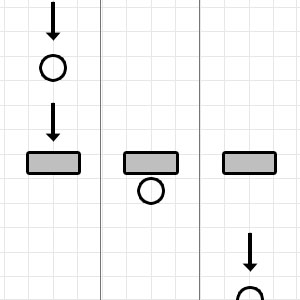
\includegraphics[scale=0.55]{tunnel.png}
	\caption{Tuneliranje (\tiny preuzeto sa \url{ https://tinyurl.com/yxjz7vga }).}
	
	\label{fig:tunnel}
\end{figure}

Tuneliranje se češće javlja kod malih objekata ili kod onih koji se brzo kreću.
U oba slučaja problem je u tome što je put koji objekat pređe između dve provere kolizije dosta veći u odnosu na veličinu objekta. 
Problem se rešava tako što se ne proverava kolizija za sâm objekat, već za celu zapreminu kroz koju je on prošao 
od prošlog trenutka provere kolizije pa do trenutnog. Na slici \ref{fig:tunnel_fix} je obojena dodatna zapremina 
koja se proverava umesto da se proverava samo objekat. 

\begin{figure}[h!]
	\centering
	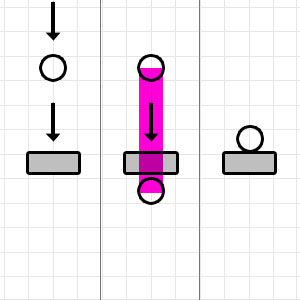
\includegraphics[scale=0.55]{tunnel_fixed.png}
	\caption{Sprečavanje tuneliranja (\tiny preuzeto sa \url{ https://tinyurl.com/yxjz7vga }).}
	
	\label{fig:tunnel_fix}
\end{figure}

Pod preciznošću se može smatrati i koliko je verodostojno predstavljen model objekta prilikom ispitivanja postojanja kolizije u odnosu 
na model koji se iscrtava.
Na slici \ref{fig:hitbox} je prikazana aproksimacija kompleksnijeg modela čoveka pomoću malog broja kvadara.
Na ovaj način dobija se prostiji ali često dovoljno dobar model za detekciju kolizije koji je značajno 
jeftiniji za upotrebu u realnom vremenu. 
Nekada se ceo model čoveka aproksimira samo jednom vertikalnom kapsulom
(uglavnom za proveru kolizije modela čoveka sa statičnom geometrijom sveta). 

\begin{figure}[h!]
	\centering
	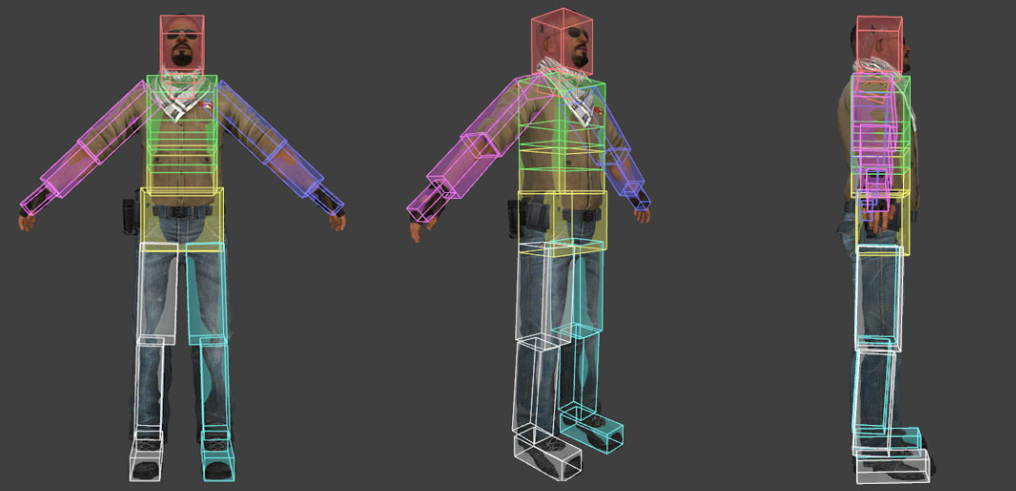
\includegraphics[scale=0.55]{hitbox.png}
	\caption{Reprezentacija modela čoveka (\tiny preuzeto sa \url{ https://tinyurl.com/yyjhzlyo }).}
	
	\label{fig:hitbox}
\end{figure}

\section{Izvršavanje na različitom hardveru}

S obzirom na to da se simulacija izvršava u diskretnim koracima,
bitan parametar prilikom izvršavanja predstavlja vremenska razlika između dva koraka.
Prevelika razlika između dva koraka je svakako nepoželjna jer je onda i prevelika razlika između dve uzastopne slike scene.

Razmotrimo naredni scenario. Potrebno je objekat pomerati duž $x$ ose za 10 jedinica svake sekunde.
Ako je interval koraka simulacije 
$p$ jednak $0.01$ sekund, onda je dovoljno da se u svakom koraku vrednost $x$ koordinate tog objekta ažurira prema sledećoj formuli:


\begin{equation}
	x:= x + 10 * 0.01
	\label{eq:prx}
\end{equation}

Zaista, kako se pri svakom koraku $x$ uveća za 0.1, a ima tačno 100 koraka u sekundi, onda će se $x$ uvećati za 10 svake sekunde.

Poželjno je da su koraci što bliži, međutim ako bi se izabrao fiksan interval koraka $p$, onda se može desiti
da se pri određenoj konfiguraciji sistema program ne izvršava dovoljno brzo. 
Ako bi razlika između dva koraka bila $q$ gde je $q > p$, 
simulacija bi u svakom koraku napredovala za $p$ jedinica unapred, te bi,
kako je $q > p$, simulacija izgledala kao usporeni snimak.
Nasuprot ovome, ako se ne bi stavila donja granica za vreme koje protekne između dva koraka onda bi na bržim računarima
simulacija bila ubrzana. 

Jedno rešenje ovog problema se sastoji u tome da se koristi 
razlika vremena proteklog između dva uzastopna koraka, u oznaci $dt$ (eng. {\em delta time}).
Korišćenjem $dt$ je moguće izvršavanje simulacije čije vreme teče konzistentno nezavisno od broja izvršenih koraka u 
jedinici vremena. Ako je hardver bolji onda će simulacija imati više koraka, odnosno više slika u sekundi, a ako je 
sporiji onda će biti manje slika u sekundi, ali vreme u simulaciji neće proticati sporije.
$dt$ bi u idealnom slučaju bilo jednako recipročnoj vrednosti broja slika u sekundi:


$$dt = \frac{1}{fps}$$
U praksi je ipak proteklo vreme između dve slike promenljivo.
Može se primetiti da dodavanjem vrednosti $dt$ promenljivoj $x$ u svakom koraku, vrednost $x$ se povećava 
za 1 svake sekunde, jer vreme svih koraka tokom jedne sekunde mora ukupno biti baš 1.
Umesto ažuriranja kao u primeru \ref{eq:prx}, sada se vrednost $x$ ažurira na sledeći način:
\begin{equation}
	\label{eq:prx2}
	x:= x + 10 * dt
\end{equation}

Kada se za ažuriranje svih objekata koristi ova formula, onda se simulacija može lako ubrzati $k$ puta
(množenjem vrednosti $dt$ sa $k$), odnosno usporiti $k$ puta (deljenjem vrednost $dt$ sa $k$).
Postavljanjem $dt$ na 0 svi objekti postaju statični. 
Na vrlo niskim fps igre postaju neprijatne za korišćenje, a čak mogu postati i nestabilne.
Dolazi do neželjenih efekata poput tuneliranja prikazanog na slici \ref{fig:tunnel}.
Tada se često postavlja gornja granica na $dt$, pa 
ako je vreme između dva koraka veće od te gornje granice onda će igra biti u usporenom snimku.
To je nešto što svakako nije poželjno, ali predstavlja prihvatljiviju varijantu od toga da dođe do pojave tuneliranja.

Pogon igara Unity deli sva ažuriranja na fiksna i opšta ažuriranja. 
Fiksna ažuriranja se koriste za promene sila nad objektima 
pošto se koraci u kojima se primenjuju neka pravila fizike izvode u fiksnim intervalima, 
dok se opšta ažuriranja koriste za operacije koje je potrebno izvršiti pre svakog iscrtavanja slike. 
Na primer, izmena korisničkog interfejsa igre spada pod opšta ažuriranja, a primena sile ili obrtnog momenta spada pod fiksna ažuriranja.
Unity izvršava fiksno ažuriranje i fizička izračunavanja 50 puta u sekundi, nezavisno od broja slika u sekundi \cite{unity}.
To znači da ako se igra izvršava na 25fps onda će biti oko dva poziva fiksnog ažuriranja na svaku iscrtanu sliku,
a ako se izvršava na 100fps tada između nekih slika neće biti nijednog fizičkog izračunavanja ni fiksnog ažuriranja.

\section{Metode za razrešavanje kolizije}
\label{sec:razresenje}

Razrešenje kolizije se sastoji od
pomeranja objekata tako da se oni više ne seku i postavljanja novih vektora brzina i sila koje deluju na objekte.
Nakon što algoritam detekcije kolizije odredi sve parove objekata koji su u koliziji, 
razrešenje kolizije svih objekata se izvodi razmatranjem svakog od parova.
Postoje dva glavna načina za razrešenje kolizija \cite{Moore}.
Jedan način je da se ubaci kruta opruga između dva objekta u koliziji.
Sila opruge se primenjuje jednako u suprotnom smeru na ta dva objekta.
Smer sile je takav da što pre razdvoji objekte. Metod sa oprugama nije težak 
za implementaciju, dobar je i za čvrsta i za fleksibilna tela, ali je problem što je računski zahtevan. 
Što je opruga kruća, potrebni su kraći vremenski koraci za fina numerička izračunavanja.

Drugi način za razrešavanje kolizije se sastoji u tome da se analitički izračunaju nova svojstva objekata u jednom koraku.
Najpre je potrebno izračunati minimalni vektor translacije. Npr. za dve sfere $s_1$ i $s_2$ to je vektor $\overrightarrow{mtv}$
određen centrima $c_1, c_2$ dve sfere čiji je intenzitet jednak razlici intenziteta zbira poluprečnika
$r_1$ i $r_2$ dve sfere i intenziteta udaljenosti centara, odnosno:
\begin{equation}
	\label{eq:mtv}
	 \overrightarrow{mtv} := \frac{{c_1 - c_2}} {\|{c_1 - c_2}\|} 
	(r_1 + r_2 - \| {c_1 - c_2} \| ) 
\end{equation}

Potom se jedna sfera translira za $ \frac{ \overrightarrow{mtv} }{ 2 }$, a druga za $ -\frac{ \overrightarrow{mtv} }{ 2 }$.
Sada sfere više nisu u koliziji, ali je potrebno da se promene njihovi vektori brzina nakon sudara.
Kada se koristi elastična kolizija onda se nove brzine računaju prema formulama:


\begin{equation}
	\label{eq:razresenje}
	\begin{split}
		{v}'_1= {v}_1-\frac{2 m_2}{m_1+m_2} \ \frac{\langle  {v}_1- {v}_2,\, {c}_1- {c}_2\rangle}{\| {c}_1- {c}_2\|^2} \ ( {c}_1- {c}_2) \\
		%\\
		{v}'_2= {v}_2-\frac{2 m_1}{m_1+m_2} \ \frac{\langle  {v}_2- {v}_1,\, {c}_2- {c}_1\rangle}{\| {c}_2- {c}_1\|^2} \ ( {c}_2- {c}_1) 
	\end{split}
\end{equation}


\noindent pri čemu su $m_1$ i $m_2$ redom mase sfera $s_1$ i $s_2$, a uglaste zagrade označavaju skalarni proizvod vektora.
Analitičko izračunavanje je glavni metod koji se koristi u pogonima igara.
On je pogodniji za jake sudare, pošto je dovoljno jednom izračunati sve promene.
Ipak, za delikatnije sudare poput tela koje je polegnuto na drugo, bolje je koristiti opruge.

% ==============================================================================
\chapter{Algoritmi za detekciju kolizije}
\label{sec:algoritmi}
% ==============================================================================

Rezultat izvršavanja algoritma detekcije kolizije je skup svih parova objekata koji su u koliziji.
U najgorem slučaju (na primer kada su svi objekti kocke na istoj poziciji) svaki objekat se seče sa svim ostalim
i tada ima $ {n\choose 2}  $ preseka, gde je $n$ broj objekata. 

Međutim, taj najgori slučaj se retko dešava u stvarnim primenama. 
Stoga, bilo bi poželjno da složenost algoritma za detekciju kolizije zavisi od broja parova objekata koji su u koliziji.
Za takve algoritme se kaže da su zavisni od izlaza, tj. njihovo vreme izvršavanja zavisi i od veličine izlaza. 
Tokom razmatranja algoritama će se podrazumevati da su svi objekti ograničavajuće kutije koje su paralelne osama,
tj. AABB. U daljem tekstu broj objekata koji se presecaju označen je sa $k$.

Pokazano je da optimalan algoritam koji pronalazi preseke $n$ AABB tela ima složenost 
$O(n \log^2 n + k)$ \cite{glavna1}. 
U praksi se obično zna u kakvim će okolnostima algoritam detekcije kolizije biti primenjen, pa 
se na osnovu toga vrši odabir postojećih ili konstruišu novi algoritmi.

\section{Osnovni algoritam}
\label{subsec:triv}

Do trivijalnog algoritma detekcije kolizije nije teško doći: za svaki element se proverava da li postoji presek sa svakim drugim elementom.
Nije teško pokazati korektnost ovog algoritma i njegova vremenska složenost je $\Theta (n^2) $ (gde je $n$ broj objekata), dok je prostorna složenost
$O(n^2)$, odnosno $\Theta(k)$ (gde je $k$ broj parova objekata koji se presecaju), pošto svaki par objekata koji je u koliziji treba sačuvati.
Na složenost vremena izvršavanja ne utiču veličina objekata, njihova brzina, ni broj parova objekata koji su u koliziji.

Algoritam je prikazan pseudokodom \ref{alg:triv}.
Glavna mana ovakvog algoritma je kvadratna vremenska složenost čak i kada nema nijedne kolizije.
Do efikasnijih algoritama može se doći particionisanjem prostora na manje potprostore, tako da
se provere kolizije vrše samo nad manjim podskupovima svih elemenata.

\begin{figure}[!h]
    \label{alg:triv}
	\begin{algorithmic}[1]
		\Procedure{OsnovnaDetekcijaKolizije}{$objekti$}
		\State $Parovi := \{ \}$
		\State $n$ := broj($objekti$)
		\For{$i := 0 $ to $n-1$}
			\For{$j$ := $i+1$ to $n$}
			\If{$objekti[i] \cap objekti[j] \neq \emptyset$}
				\State $Parovi:=Parovi \cup \{i, j\}$
			\EndIf		
		\EndFor
		\EndFor
		\State \textbf{return} $Parovi$
		\EndProcedure
    \end{algorithmic}
\caption{Osnovni algoritam detekcije kolizije}
\end{figure}

\section{Oktri}
\label{subsec:octree}

\textbf{Oktri} (eng. {\em Octree}) je prostorna struktura podataka koja se koristi za rekurzivno deljenje trodimenzionog prostora na oktante.
Suštinski, oktri je stablo kod koga svaki unutrašnji čvor ima tačno osmoro dece,
što odgovara podeli prostora koji odgovara tom unutrašnjem čvoru na osam podkocki (oktanata).
U listovima se čuvaju objekti koji pripadaju oktantu koji taj list predstavlja.
%Oktri može biti tako implementiran da predstavlja i beskonačan prostor.
Na slici \ref{fig:oct} je prikazan način particionisanja trodimenizionog prostora korišćenjem oktrija.

Objekti se ubacuju u stablo počevši od korena idući rekurzivno kroz one oktante kojima objekat pripada,
sve dok se ne stigne do lista.
Pritom, postoji namenska konstanta $c$ koja sadrži vrednost najvećeg dozvoljenog broja elemenata koji list stabla može da sadrži.
Kada se prekorači taj maksimum $c$, onda list postaje unutrašnji čvor, njegov potprostor se deli 
na osam podoktanata u koje se prebacuju objekti koje je sadržao.
Potrebno je izabrati još jednu konstantu $h$ koja predstavlja maksimalnu dubinu stabla oktrja.
Ukoliko maksimalna dubina stabla ne bi bila ograničena onda u slučaju da se ubacuje $n$ identičnih objekata (gde je $n > c$)
stablo bi se beskonačno rekurzivno delilo pokušavajući da podeli tih $n$ objekata u različite listove 
tako da svaki ima manje ili jednako $c$ objekata u sebi. 
Pošto to nije uvek moguće izvesti, konstanta $h$ zaustavlja takve podele stabla.

Parovi objekata koji su u koliziji se onda mogu pronaći na sledeći način:
kada se objekat ubaci u list, proverava se da li on ima presek sa objektima koji su već
ubačeni u taj list i svi parovi koji se seku se prijave.
Drugi način da se odrede svi parovi objekata u koliziji se sastoji u tome da se prvo svi objekti smeste u oktri, 
pa da se naknadno prođe kroz sve listove i za svaka dva objekta koji pripadaju istom listu proveri da li su u koliziji.
Treba primetiti da je složenost provere kolizija kvadratna po broju elemenata u listu.
To ipak nije problem kada su elementi pretežno uniformno raspoređeni po prostoru, što je često 
i slučaj jer se uglavnom ne dopušta njihovo trajno presecanje. 

\begin{figure}[!h]
    \label{alg:octree}
	\begin{algorithmic}[1]
		\Procedure{OktriDetekcijaKolizije}{$objekti$, $korenOktri$}
		\State $Parovi := \{ \}$
		\For{$obj$ in $objekti$}
			\State DodajUČvor($obj$, $korenOktri$, $Parovi$)
		\EndFor
		\State \textbf{return} $Parovi$
		\EndProcedure

		\Procedure{DodajUČvor}{$objekat$, $\check{c}vor$, $Parovi$}
		\If{$\check{c}vor$ nije list}
			\State DodajNaniže($objekat$, $\check{c}vor$, $Parovi$)
			\State \textbf{return}
		\EndIf		

		/*{$\check{c}vor.elementi$ je vektor elemenata u listu oktrija}*/
		\For{$element$ in $\check{c}vor.elementi$}
			\If{$objekat \cap element \neq \emptyset$}
				\State $Parovi := Parovi \cup \{objekat, element\}$
			\EndIf		
		\EndFor

		\State dodaj $objekat$ u $\check{c}vor.elementi$

		\If{$\check{c}vor$ na maksimalnoj dubini ili broj($\check{c}vor.elementi$) <= maksimum}
			\State \textbf{return}
		\EndIf	

		\State podeli $\check{c}vor$ na podoktante

		\For{$element$ in $\check{c}vor.elementi$}
			\State DodajNaniže($element$, $\check{c}vor$, $Parovi$)
		\EndFor

		\State obriši vektor $\check{c}vor.elementi$

		\EndProcedure

		\Procedure{DodajNaniže}{$objekat$, $\check{c}vor$, $Parovi$}
		\For{$podoktant$ in $\check{c}vor$}
			\If{$podoktant \cap objekat \neq \emptyset$}
				\State DodajUČvor($objekat$, $podoktant$, $Parovi$)
			\EndIf	
		\EndFor
		\EndProcedure
	\end{algorithmic}
	\caption{Oktri detekcija kolizije (sa duplikatima)}
\end{figure}

Ukoliko se razmatra tačkasti objekat, opisani postupak umetanja radi korektno,
ali se postavlja pitanje šta raditi sa većim objektima koji pripadaju većem broju oktanata.
Jedno rešenje bi bilo da se objekat ubaci u svaki oktant kome bar delimično pripada.
Bitan problem sa tim rešenjem je taj što ako je u pitanju veliki objekat, onda će on pokriti mnoge oktante, njihove 
podoktante i tako rekurzivno. 
Tada veliki broj listova mora da pamti taj objekat, tj. njegovu referencu ili indeks u nekom nizu.
To nije velika smetnja kada su svi objekti sličnih veličina, ali ako 
nisu, onda i memorijska i vremenska složenost mogu eksplodirati.
Ovakav oktri će se u daljem tekstu nazivati \textbf{oktri sa duplikatima} (eng. {\em octree with duplicates}). 
Oktri sa duplikatima prikazan je pseudokodom \ref{alg:octree}.

Drugo rešenje bi bilo da se dopusti i unutrašnjim čvorovima stabla da čuvaju objekte.
Kada neki objekat seče više od jednog oktanta nekog unutrašnjeg čvora $U$, tada se on ne ubacuje 
u podoktante čvora $U$, nego se pamti u čvoru $U$. Time se može značajno uštedeti na memoriji i vremenu izvršavanja.
U daljem tekstu će se ovakav oktri nazivati \textbf{oktri bez duplikata} (eng. {\em octree without duplicates}).
Međutim, i za tako izmenjen oktri postoje nezgodne situacije kada se pogoršava vreme izvršavanja.
Ako svi objekti seku više od jednog podoktanta korenog čvora, onda svi moraju biti sačuvani u njemu. 
U tom slučaju se mora proveriti kolizija svih parova od $n$ objekata, što je ekvivalentno osnovnom kvadratnom algoritmu.

Očekivano vreme izvršavanja za izgradnju oktrija je $O(n \log n)$, gde je $n$ broj objekata.
Očekivano vreme potrebno za pronalazak svih kolizija je $O(n \log n + k)$, gde je $k$ broj objekata koji su u koliziji.

Parametri oktrija $c$ i $h$  utiču značajno na njegovu efikasnost u praksi. 
Iako broj provera u listu raste kvadratno sa $c$, to nije problem za relativno male vrednosti $c$, i često je bolje 
imati nešto veći broj elemenata u listu nego da se stablo više particioniše i duže putuje kroz njega.
Ti parametri su promenljivi u projektu i dobre vrednosti ovih parametara mogu se odrediti njihovim podešavanjem u realnom vremenu,
o čemu će biti reči kasnije.

Kada se svi objekti kreću, onda se u svakom koraku simulacije  gradi novi oktri u
koga se ubacuju svi elementi i usput otkrivaju kolizije.
Čest je slučaj kada je veliki broj objekata statički pa je tada dovoljno jednom izgraditi oktri za njih, a za objekte koji se kreću u svakom koraku 
izvršiti detekciju kolizije njihovim ponovnim ubacivanjem u stablo. Time se smanjuje vreme izvršavanja upita 
kolizije jednog objekta koji se kreće sa $n$ statičkih objekata sa $O(n)$ na očekivanih $O(\log n)$.

\begin{figure}[h!]
	\centering
	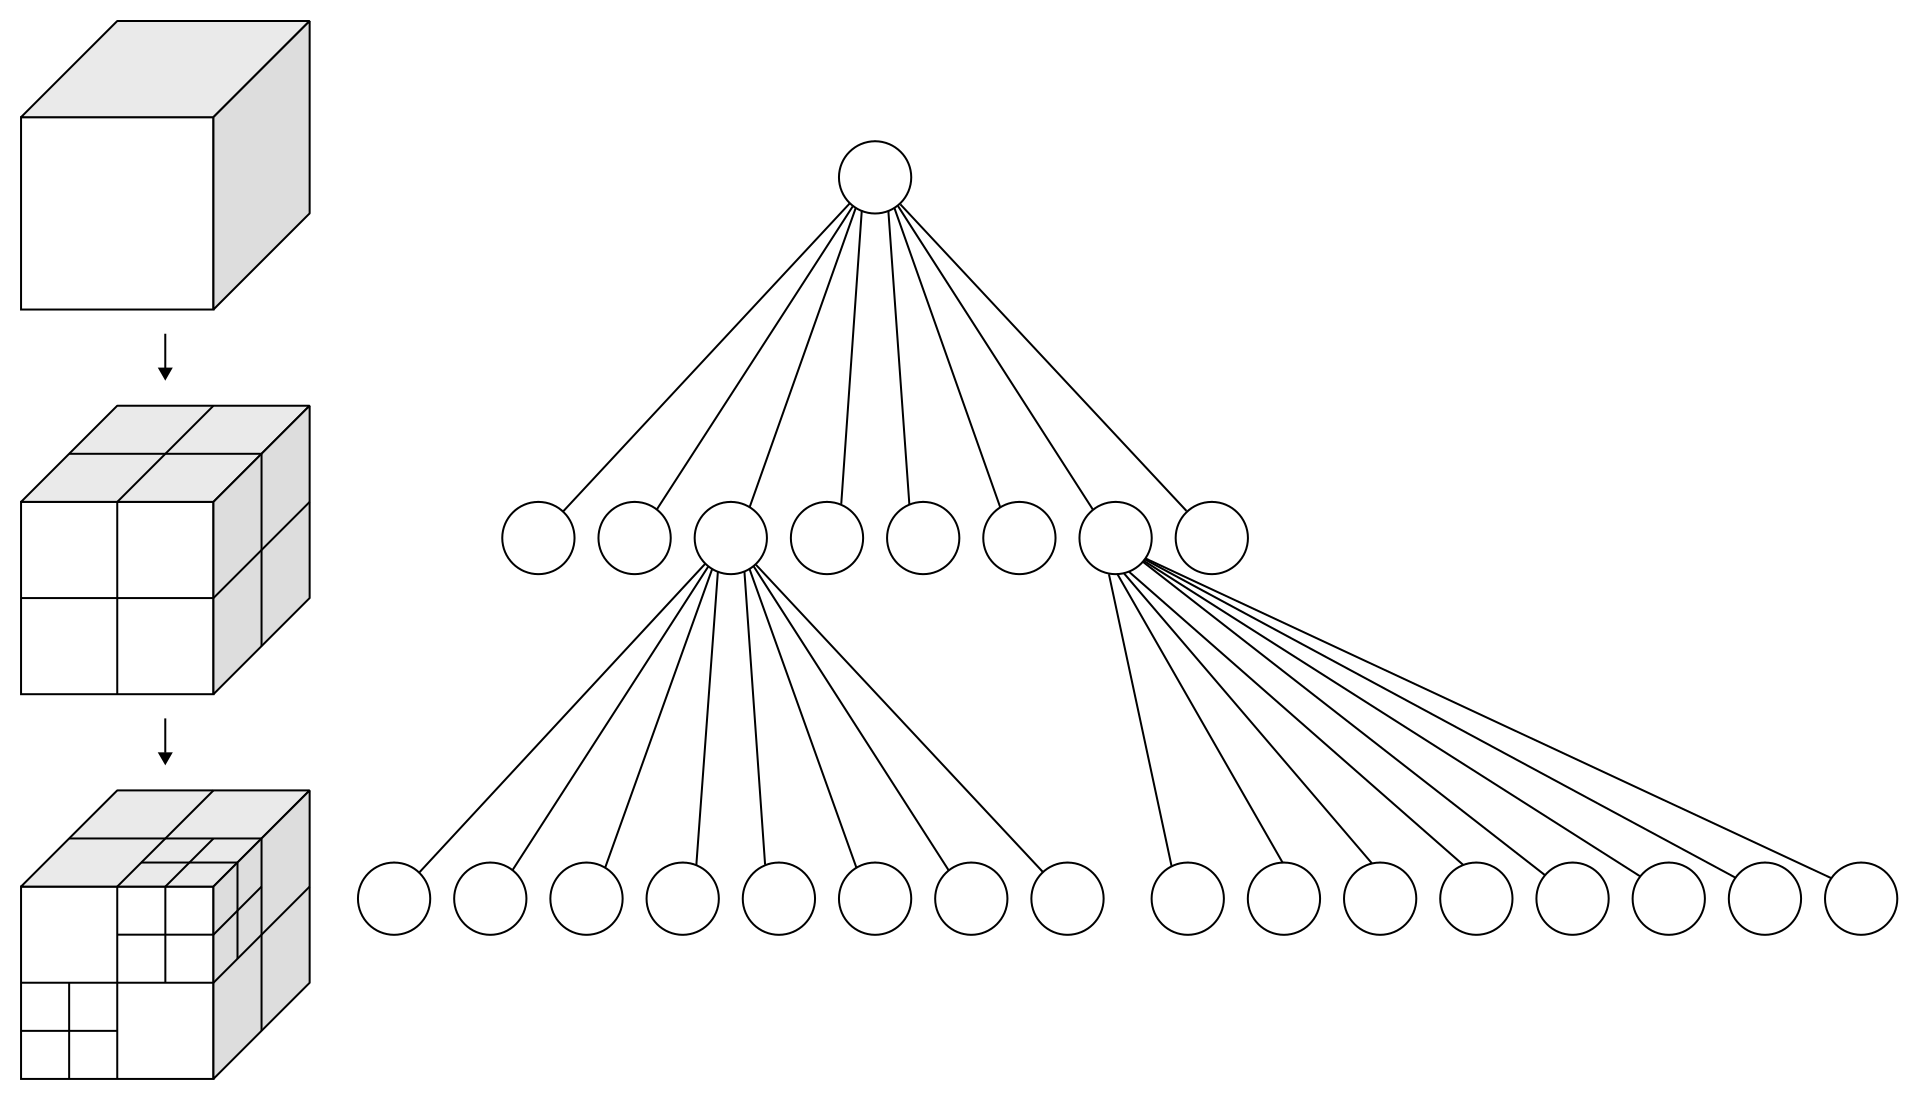
\includegraphics[scale=0.22]{octree.png}
	\caption{Rekurzivno deljenje kocke na oktante (\tiny preuzeto sa \url{ https://tinyurl.com/y4ep88wa }).}
	
	\label{fig:oct}
\end{figure}

\section{Briši i odseci}
\label{subsec:sap}

\textbf{Briši i odseci} (eng. {\em sweep and prune}), skraćeno \textbf{SAP}, je alternativa tehnikama detekcije kolizije 
zasnovanim na prostornom particionisanju.
SAP je algoritam široke faze koji projektuje sve AABB
na bazne ose (u trodimenzionalnom slučaju to je tri skupa projekcija) pa sortira projekcije da bi odredio preseke AABB.
Ako se po sve tri ose projekcije nekog para AABB seku, onda se taj par AABB seče i u prostoru.

Ako je potrebno naći sve parove objekata koji su u koliziji samo u jednom vremenskom trenutku onda ovaj metod ne predstavlja neko poboljšanje u odnosu na druge.
Moć briši i odseci algoritma je u tome što koristi svojstvo vremenske koherentnosti.
Objekti se ne teleportuju nasumično kroz prostor nego se postepeno kreću. 
Zbog toga je za svaku iteraciju moguće inkrementalno ažurirati parove objekata koji su u koliziji.
To se može postići na sledeći način: održavaju se tri sortirana niza, pri čemu svaki od njih sadrži $2n$ elemenata, gde je $n$ broj objekata.
Svaki niz sadrži po dva elementa za projekciju svakog AABB po jednoj osi: jedan element je početak,
odnosno teme sa manjom koordinatom, a drugi je kraj projekcije, tj. teme sa većom koordinatom. 

Na slici \ref{fig:sap} je prikazana projekcija četiri objekta na jednu osu. 
Tačka $b_i$ označava početak, a $e_i$ kraj projekcije $i$-tog objekta.
U prvom momentu $e_3$ se nalazi desno od $b_4$, što posmatranjem projekcije na jednoj osi govori da su njihovi AABB možda u koliziji.
Potrebno je proveriti i ostale (ovde samo još jednu) osu sa projekcijama da bi se utvrdilo da li se stvarno seku.
Svi parovi objekata koji su u koliziji se zapamte u kolekciji parova kolizija, u ovom slučaju to je samo par $(3, 4)$.
U sledećem koraku se proverava da li je neki par koji je bio u koliziji prestao da bude, 
odnosno da li je možda neki par objekata koji prethodno nije bio u koliziji sada u koliziji.
Nakon pomeranja objekata potrebno je ažurirati projekcije objekata tako da nizovi i dalje ostanu sortirani.
Prilikom sortiranja nizova se u stvari dodaju i uklanjaju kolizije.

Za održavanje sortiranosti se koristi sortiranje umetanjem (eng. {\em insertion sort}) 
pošto ovaj algoritam sortiranja pokazuje veoma dobre osobine za skoro sortirane nizove.
Tokom sortiranja niza posmatraju se elementi koji predstavljaju projekcije sleva (početak niza) nadesno i za svaki element $A$ se proverava da li treba da se elementi $B_i$ levo od $A$
pomere za jednu poziciju udesno. Postoje dva uslova koji utiču na postojanje kolizija:
\begin{itemize}  
	\item Ako je $A$ krajnja tačka projekcije, a tačka $B_i$ je početna onda se par ovih objekata izbacuje iz kolekcije parova kolizije.
	Naravno, prave kolizije nije moralo ni biti u slučaju da se projekcije na ostale ose ne seku, 
	pa tada izbacivanje ovog para iz kolekcije neće imati nikakvog efekta.
	\item Ako je $A$ početna tačka projekcije, a tačka $B_i$ je krajnja onda se vrši provera da li se seku projekcije na ostale ose (AABB upit) i ako se seku
	onda se par odgovarajućih objekata dodaje u kolekciju parova kolizije.

\end{itemize}  

Parovi objekata koji imaju presek se čuvaju u heš mapi, pa je dodavanje novih parova i uklanjanje postojećih parova objekata koji imaju presek brzo.
Za inicijalizaciju kolizija može se koristiti isti postupak koji se koristi za održavanje sortiranosti niza.
Međutim, to znači da je potrebno sortirati prvobitni niz (koji može biti veoma daleko od sortiranog niza) algoritmom sortiranja umetanjem.
Umesto toga je bolje prvi korak realizovati nekim drugim algoritmom detekcije kolizije, na primer pomoću oktrija.

\begin{figure}[h!]
	\centering
	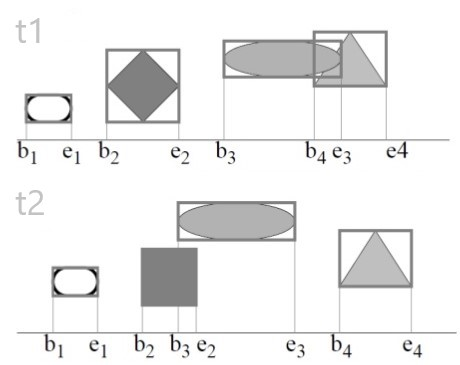
\includegraphics[scale=0.8]{sap.jpg}
	\caption{Projekcije tela na jednu osu u dva koraka (\tiny preuzeto sa \url{ https://tinyurl.com/y3zetsmj }).}
	
	\label{fig:sap}
\end{figure}

Umesto da se AABB upiti vrše svaki put iznova, moguće je da se čuvaju informacije o presecima 
na svakoj osi. To zahteva $O(n^2)$ memorije ali smanjuje posao prilikom zamena \cite{sap}. 

Potrebno je definisati metode za inicijalizaciju, napraviti strukture koje će čuvati parove preseka,
kao i strukturu za tačke projekcije (sadrži svoju vrednost na osi, da li je početna ili krajnja tačka projekcije i od kog objekta potiče)
i indeks u polaznoj kolekciji objekata.
Srž SAP algoritma je prikazana pseudokodom \ref{alg:SAP}. 
U prikazanoj proceduri se ažurira kolekcija $Parovi$ koja sadrži parove objekata koji imaju presek. 
Kolekcija $Parovi$ je implementirana kao heš skup celobrojnih indeksa tih parova u nizu $objekti$.

\begin{figure}[!h]
    \label{alg:SAP}
	\begin{algorithmic}[1]
		\Procedure{SAPSortirajOsuProjekcije}{$osa$, $objekti$} 
		\For{$i$ :=1 to $2 \cdot osa.brojTa\check{c}aka$}
			\State $trenutna$ :=  $osa[i]$
			\State $vrednost$ := $trenutna.vrednost$
			\State $j$ := $i$ -1
			\While{$j$ >= 0 and $osa[j].vrednost$ > $vrednost$}
				\State $pomeriti$ := $osa[j]$

				\If{$pomeriti$ je početna and $trenutna$ je krajnja tačka projekcije}

					\State $Parovi := Parovi \setminus \{pomeriti.indeks, trenutna.indeks\}$
				\EndIf		

				% todo mozda bools
				\If{$pomeriti$ je krajnja and $trenutna$ je početna tačka projekcije}
					\If{$objekti[pomeriti.indeks] \cap objekti[trenutna.indeks] \neq \emptyset$}
						\State $Parovi := Parovi \cup \{pomeriti.indeks, trenutna.indeks\}$
					\EndIf		
				\EndIf

				\State $j := j - 1$
			\EndWhile
		\EndFor
		\State \textbf{return} $Parovi$
		\EndProcedure
	\end{algorithmic}
	\caption{Glavni deo briši i odseci algoritma detekcije kolizije}
\end{figure}

Ovaj metod pokazuje najbolje performanse kada su objekti uniformno raspoređeni, dok mu je ponašanje lošije kada je
prisutan klaster većine objekata na nekoj osi, što vodi kvadratnoj složenosti po broju objekata \cite{sap}.

Prilikom evaluacije pokazuje se da najveći uticaj na performanse ima brzina kretanja objekata.
U slučaju kada se objekti brzo kreću, pomeraji objekata su veliki i potrebno je vršiti brojnije zamene njihovih pozicija u sortiranom nizu,
što vodi jakom usporavanju algoritma.
Tada svaka tačka projekcije u nizovima mora 
da se poredi sa većim brojem ostalih što dovodi do ispoljavanja kvadratne vremenske složenosti algoritma sortiranja umetanjem.
Ipak, kada se svi objekti polako kreću, onda je mali broj pomeraja u nizu, i vreme izvršavanja algoritma je praktično 
linearno, što omogućava veći broj pokretnih objekata i kraće vreme izvršavanja od ostalih razmatranih algoritama.

\section{Ćelije i portali}
\label{subsec:cells}

Pravljenje dodatnog modela particionisanja prostora samo za detekciju kolizije nije uvek neophodno.
Postojeća hijerarhijska organizacija koja se koristi za renderovanje slika je nekad sasvim dovoljna.
Jedan primer takve organizacije predstavlja \textbf{graf scene} (eng. {\em scene graph}).
Graf scene je struktura podataka koja se koristi u svrhe logičke i prostorne organizacije objekata na sceni.

\textbf{Metod ćelija i portala} (eng. {\em cells and portals}) je organizaciona struktura koja se može upotrebiti kao graf scene
i istovremeno koristiti kao struktura prostornog particionisanja koja se koristi za detekciju kolizije.
Ova metoda je razvijena za potrebe renderovanja sistema arhitekturalnog prolaska. 
Za ove sisteme je karakteristično okruženje koje se sastoji od velikog broja prostorija, tako da u svakom trenutku
većina objekata koji se nalaze u zarubljenoj četvorostranoj piramidi pogleda (eng. {\em frustum})
nije vidljivo, pošto je skoro sva vidljiva geometrija unutar trenutne sobe u kojoj se posmatrač nalazi.
Metoda ćelija i portala deli svet u regije, odnosno ćelije, i delove koji ih spajaju, odnosno portale.
Dakle u slučaju zgrada, sobe odgovaraju ćelijama, a vrata odgovaraju portalima. 

Renderovanje scene koja je podeljena u ćelije i portale počinje od one ćelije u kojoj se nalazi posmatrač. 
Nakon što je početna ćelija obrađena, proces renderovanja se poziva rekurzivno
za susedne ćelije čiji su portali vidljivi posmatraču. 
Pravi se presek novih portala sa pogledom trenutnog portala čime se sužava vidljivost scene.
Rekurzija se zaustavlja kada je presek novog portala sa trenutnim prazan, ili kada su posećene sve dostupne susedne ćelije \cite{glavnaKnjiga}.
Primer renderovanja stana predstavljenog preko ćelija i portala je dat na slici \ref{fig:cellsRooms}.

\begin{figure}[h!]
	\begin{center}
	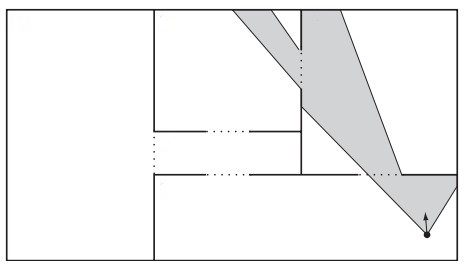
\includegraphics[scale=1]{cellsRooms.jpg}
	\end{center}
	\caption{
	Osenčen region predstavlja ono što posmatrač vidi. 
	Potrebno je da se renderuju samo tri od šest ćelija (\tiny preuzeto sa \cite{glavnaKnjiga}). }
	\label{fig:cellsRooms}
\end{figure}

Ista struktura ćelija i portala može se iskoristiti i za brzu detekciju kolizije. 
Objekti su pridruženi ćeliji u kojoj im se nalazi centar. Kada se objekti kreću vrši 
se provera da li je objekat napustio svoju ćeliju. Ako jeste, onda se pravi presek tog objekta
sa susednim ćelijama da bi se saznalo gde je otišao. 

Kada se vrši detekcija kolizije između pokretnih objekata, za svaki objekat X 
potrebno je samo proveriti objekte koji su dodeljeni istoj ćeliji kao i X, i u slučaju
da X preseca neki portal, uraditi i proveru sa objektima koji su u ćeliji sa druge strane tog portala \cite{cells}.
Primer detekcije kolizije pokretnih objekata dat je na slici \ref{fig:cellsObj}.
Traženje preseka objekata u okviru jedne ćelije zahteva kvadratni broj operacija u odnosu na broj objekata u toj ćeliji.
Algoritam detekcije kolizije pomoću ćelija i portala prikazan je pseudokodom \ref{alg:cell}.
Za konstrukciju ćelija i portala uglavnom se koristi algoritam 
\textbf{binarnog particionisanja prostora} (eng. {\em binary space partitioning}).

\begin{figure}[!h]
    \label{alg:cell}
	\begin{algorithmic}[1]
		\Procedure{ĆelijeIPortaliNađiKolizije}{} 
		\State $Parovi := \{ \}$
		\For{$\acute{c}elija$ in $\acute{c}elije$}
			\State $ParoviU\acute{C}eliji$ := OsnovnaDetekcijaKolizije($\acute{c}elija.objekti$)
			\State $Parovi:=Parovi \cup ParoviU\acute{C}eliji$
		\EndFor
		\State \textbf{return} $Parovi$
		\EndProcedure
	\end{algorithmic}
	\caption{Detekcija kolizije pomoću strukture ćelija i portala}
\end{figure}

\begin{figure}[h!]
	\centering
	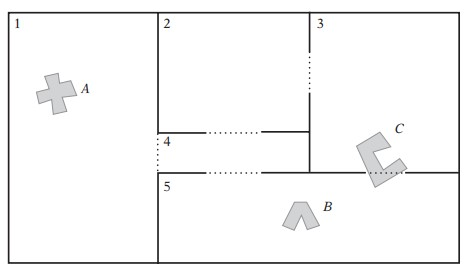
\includegraphics[scale=1]{cellsObj.jpg}
	\caption{ Objekti B i C redom u potpunosti i delimično pripadaju istoj ćeliji, pa se moraju međusobno testirati na presek,
	 dok za objekat A nije potrebno izvršiti testiranje ni sa jednim drugim objektom (\tiny preuzeto sa \cite{glavnaKnjiga}). }
	
	\label{fig:cellsObj}
\end{figure}

Ova metoda daje najbolje rezultate kada svaka ćelija ima približno isti broj objekata i kada je 
broj ćelija proporcionalan broju objekata.
Takođe, što su portali manji to će se brže zaustaviti rekurzija.
Tada se velik broj objekata može podeliti u ćelije tako da u svakoj ćeliji bude mali broj objekata,
pa kvadratni broj provera u okviru jedne ćelije neće doći do izražaja.
Ova metoda se ne koristi u modernim igarama (pre svega zbog pretpostavke da se radi o sobama sa vratima) i zato nije evaluirana u poglavlju \ref{sec:evaluacija},
ali je predstavljena zbog toga što je odlična u scenarijima za
koje je zamišljena i daje nov način razmatranja konstrukcije rešenja za problem detekcije kolizije.

% ==============================================================================
\chapter{Implementacija}
\label{sec:implementacija}
% ==============================================================================

Jedno od prvih pitanja koje je bilo postavljeno na početku rada na ovoj temi odnosilo se na to 
u kom okruženju ima najviše smisla implementirati algoritme detekcije kolizije.
Tri glavna kandidata koja su razmatrana su OpenGL, Unity i Unreal Engine.

I Unity i Unreal su pogoni igara pa samim tim imaju sve što je neophodno da 
bi se započeo razvoj igre ili neke druge aplikacije.
Unreal pruža mogućnost implementiranja preko shema (eng. {\em blueprints}),
putem programskog jezika C\texttt{++} ili njihovom mešavinom.
Unity omogućava implementiranje putem programskog jezika C\texttt{\#} ili unityscript,
koji ima sintaksu nalik jeziku JavaScript. Unityscript polako izlazi iz upotrebe, i 
sva nova dokumentacija podrazumeva korišćenje jezika C\texttt{\#}.
Jezik C\texttt{\#} u odnosu na C\texttt{++} često omogućava kraće vreme implementacije nekog rešenja,
međutim postoji cena toga - nešto sporije vreme izvršavanja.
To "nešto" je uglavnom moguće ignorisati, prateći citat Donalda Knuta 
"Prevremena optimizacija je koren svog zla u programiranju".
Ipak, u slučaju programa čije su performanse od kritičnog značaja, npr. kao što je 
slučaj sa operativnim sistemima i pogonima igara, to usporenje se ne može tolerisati.
%https://en.wikipedia.org/wiki/List_of_game_engines - kako referenca za ovo
Zato su danas praktično svi pogoni 3D igara implementirani u jeziku C\texttt{++}.

Upravo zbog raznih funkcionalnosti koje pogoni igara pružaju i zbog njihove masivnosti nisu izabrani
za osnovu implementacije ovog projekta. Oni već imaju integrisanu fiziku, detekciju 
i razrešenje kolizije. Tako bi uobičajeni kanali implementacije u njima 
bili previše indirektni za funkcionalnost koja čini srž celog sistema.
Zbog navedenih razloga je projekat napravljen korišćenjem OpenGL pomoćne 
biblioteke FreeGLUT  koja ima skroman skup pomoćnih
funkcija od kojih je većina usmerena na grafiku i vrlo su niskog nivoa.

Ovaj projekat ne implementira algoritme detekcije kolizije u izolaciji pošto 
se oni ni neće koristiti bez ostalih komponenti kao što su iscrtavanje, ažuriranje pozicije i brzine objekata,
upravljanje ulazima korisnika i razrešenje kolizije.

\section{FreeGLUT}

GLUT je biblioteka pomoćnih funkcija za OpenGL programe.
GLUT je prvobitno napisana da bi se podržali primeri programa u knjizi "OpenGL:
vodič za programiranje", poznatijoj pod nazivom "Crvena Knjiga" (eng. {\em "the Red Book"}).
FreeGLUT je alternativa otvorenog koda za GLUT (eng. {\em OpenGL Utility Toolkit}). 
GLUT se ne razvija od 1998. godine, pa je još 1999. započet projekat FreeGLUT  koji 
se razvija do danas \cite{freeglut}. 

Biblioteka FreeGLUT se stara o pravljenju prozora, obrađivanju događaja kroz glavnu petlju,
a takođe su dostupne i standardne funkcije OpenGL-a koje se koriste
za iscrtavanje poput glTranslatef, glScalef, glLightf, glMaterialfv, glViewPort, itd.
Za odgovore na događaje pritiskanja tastera, puštanja tastera i pomeraja miša
FreeGLUT propisuje korišćenje funkcija povratnog poziva  (eng. {\em callback function}) koje je potrebno implementirati.
FreeGLUT se ne stara o tome da li je u nekom trenutku neko dugme pritisnuto, 
koliki je pomeraj miša, niti ga automatski iznova pozicionira, ali barem pruža 
funkcije koje su neophodne da bi se to ostvarilo.

\section{Arhitektura}

Glavne komponente programa su:
\begin{itemize}
	\item komponenta za iscrtavanje,
	\item komponenta za rukovanje ulazima korisnika,
	\item centralna komponenta - poziva sve ostale komponente i stara se o vremenskim koracima,
	\item kontroler komponenta za upravljanje parametrima algoritama,
	\item komponenta za merenje performansi,
	\item komponenta za ažuriranje brzine i pozicije objekata.
\end{itemize}

U nastavku teksta će biti više reči o svakoj od pomenutih komponenti pojedinačno.

\begin{figure}[h!]
	\centerfloat
% https://online.visual-paradigm.com/w/jllvezfo/diagrams.jsp#diagramlist:open&mode=Local
% \includegraphics[trim=left bottom right top, clip]
	% 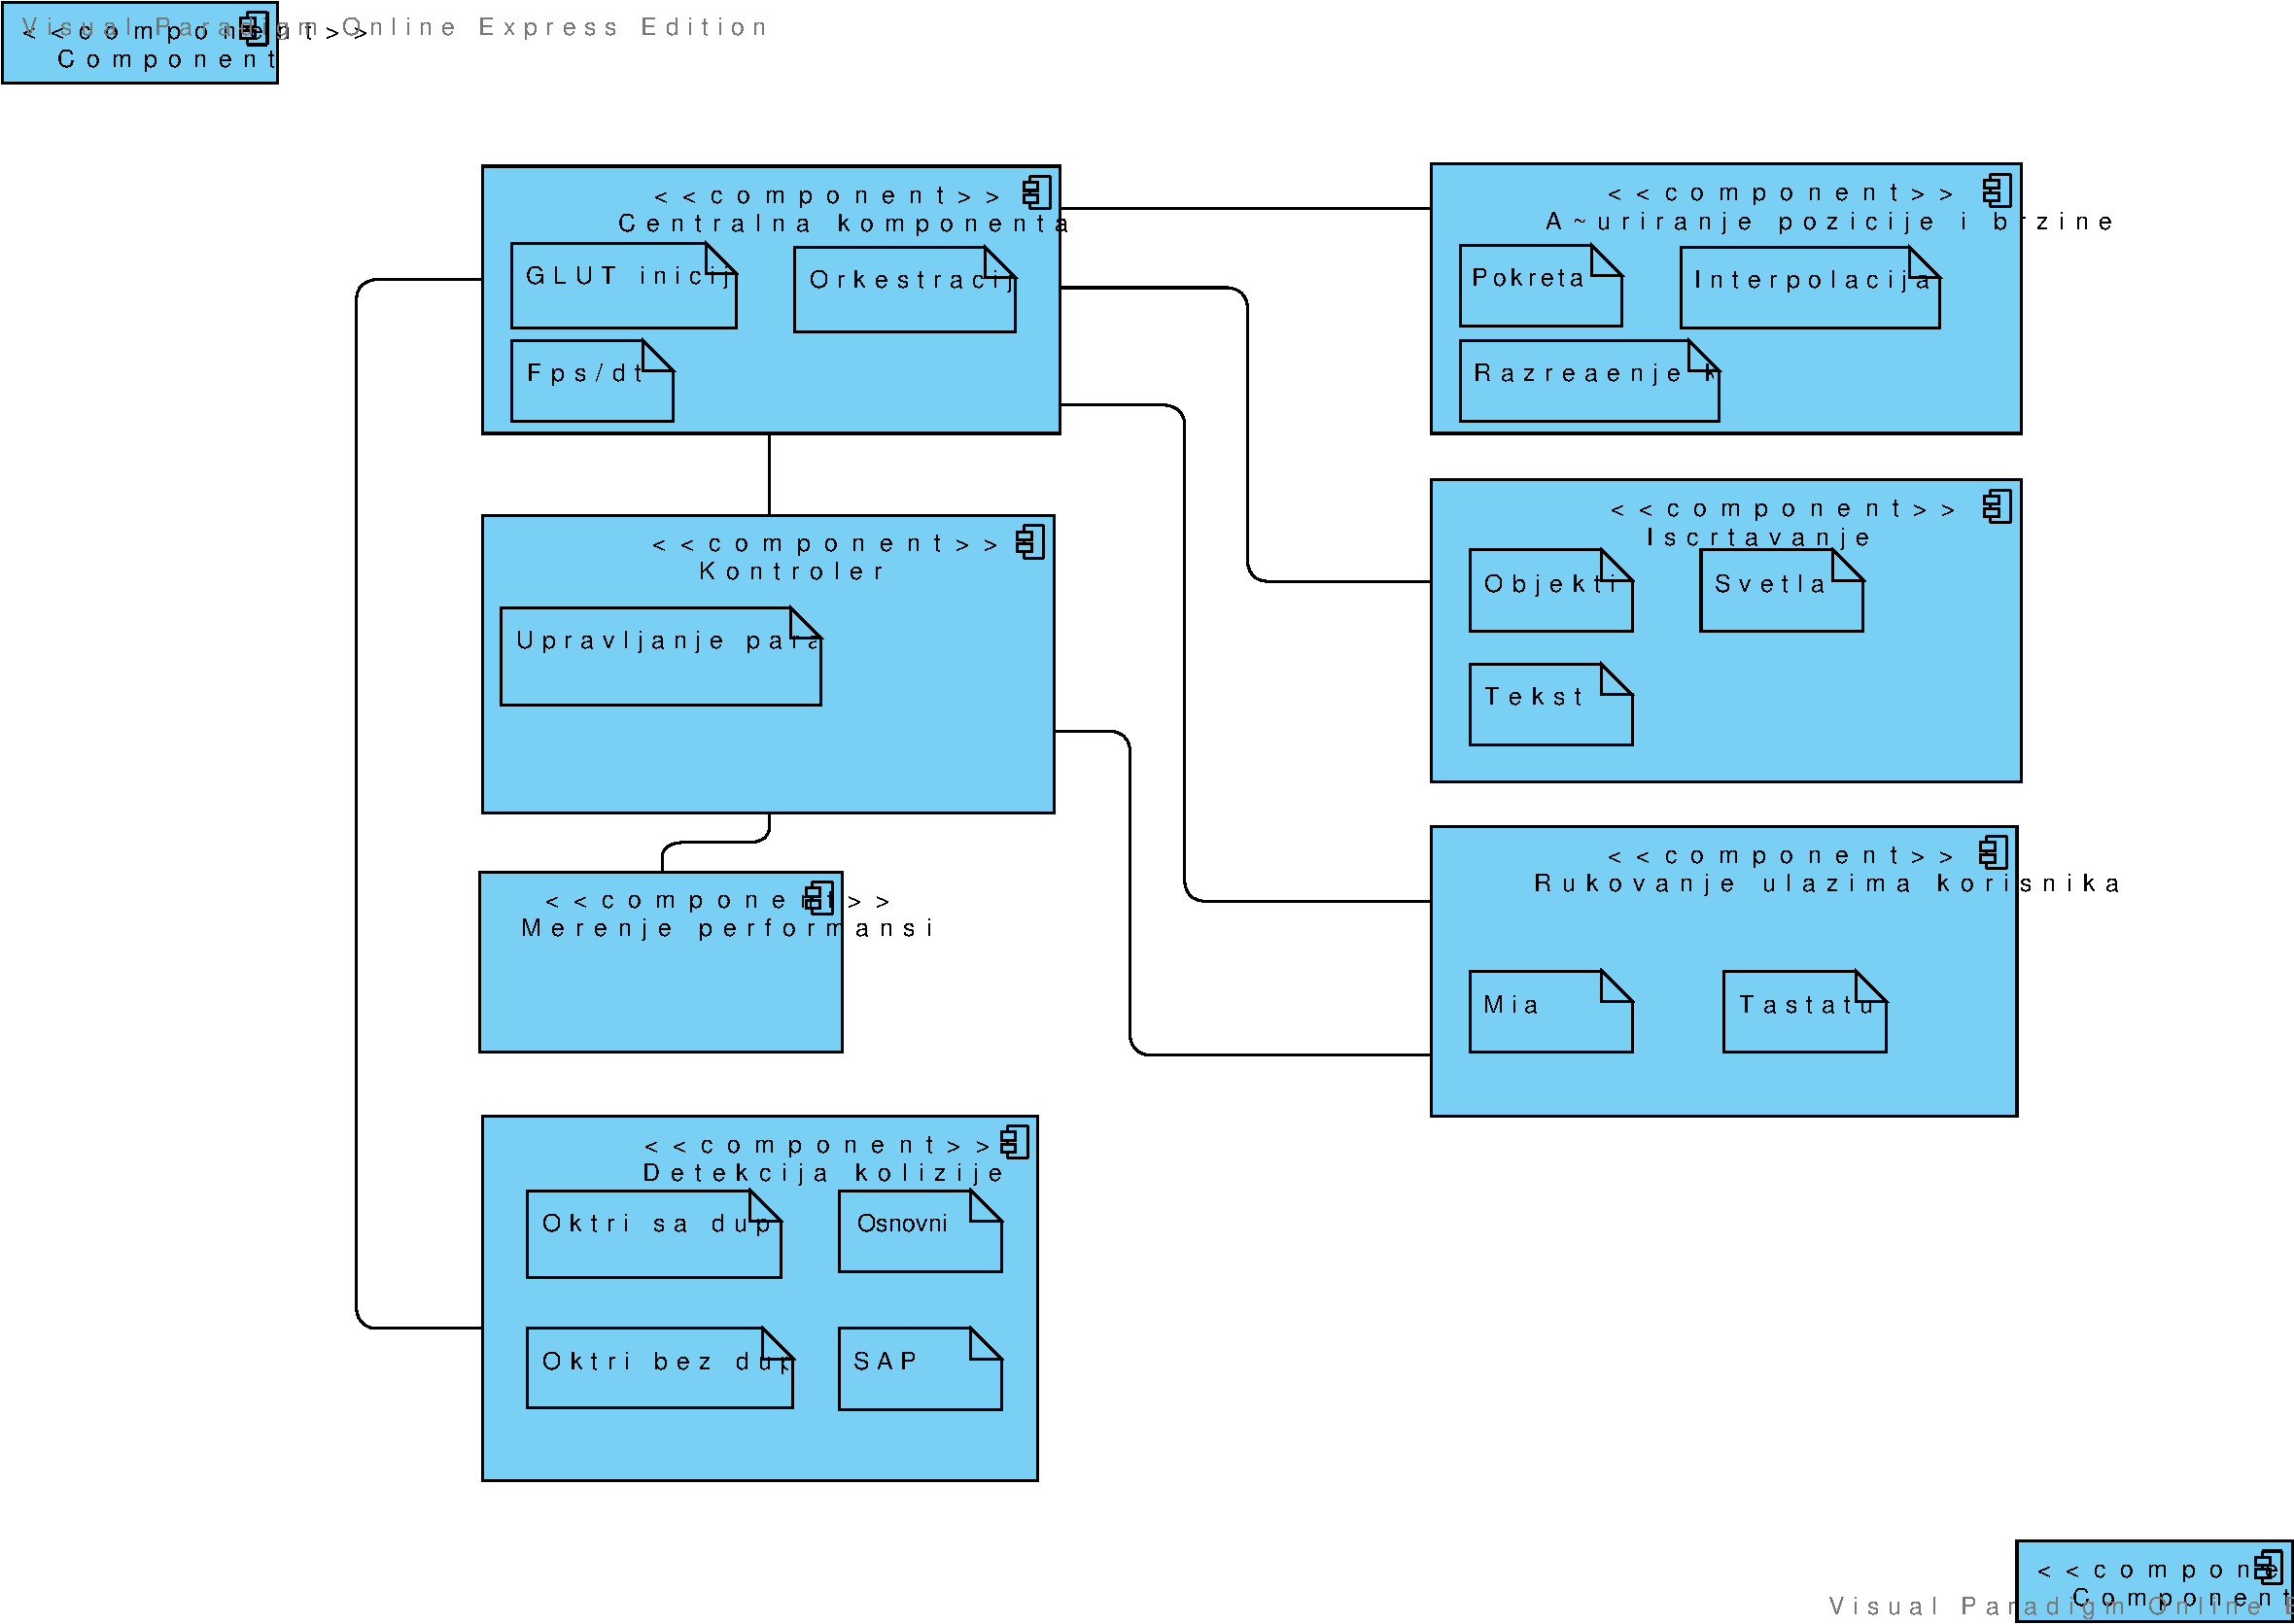
\includegraphics[trim=150 50 100 50,clip,scale=0.6]{architecture.pdf}
	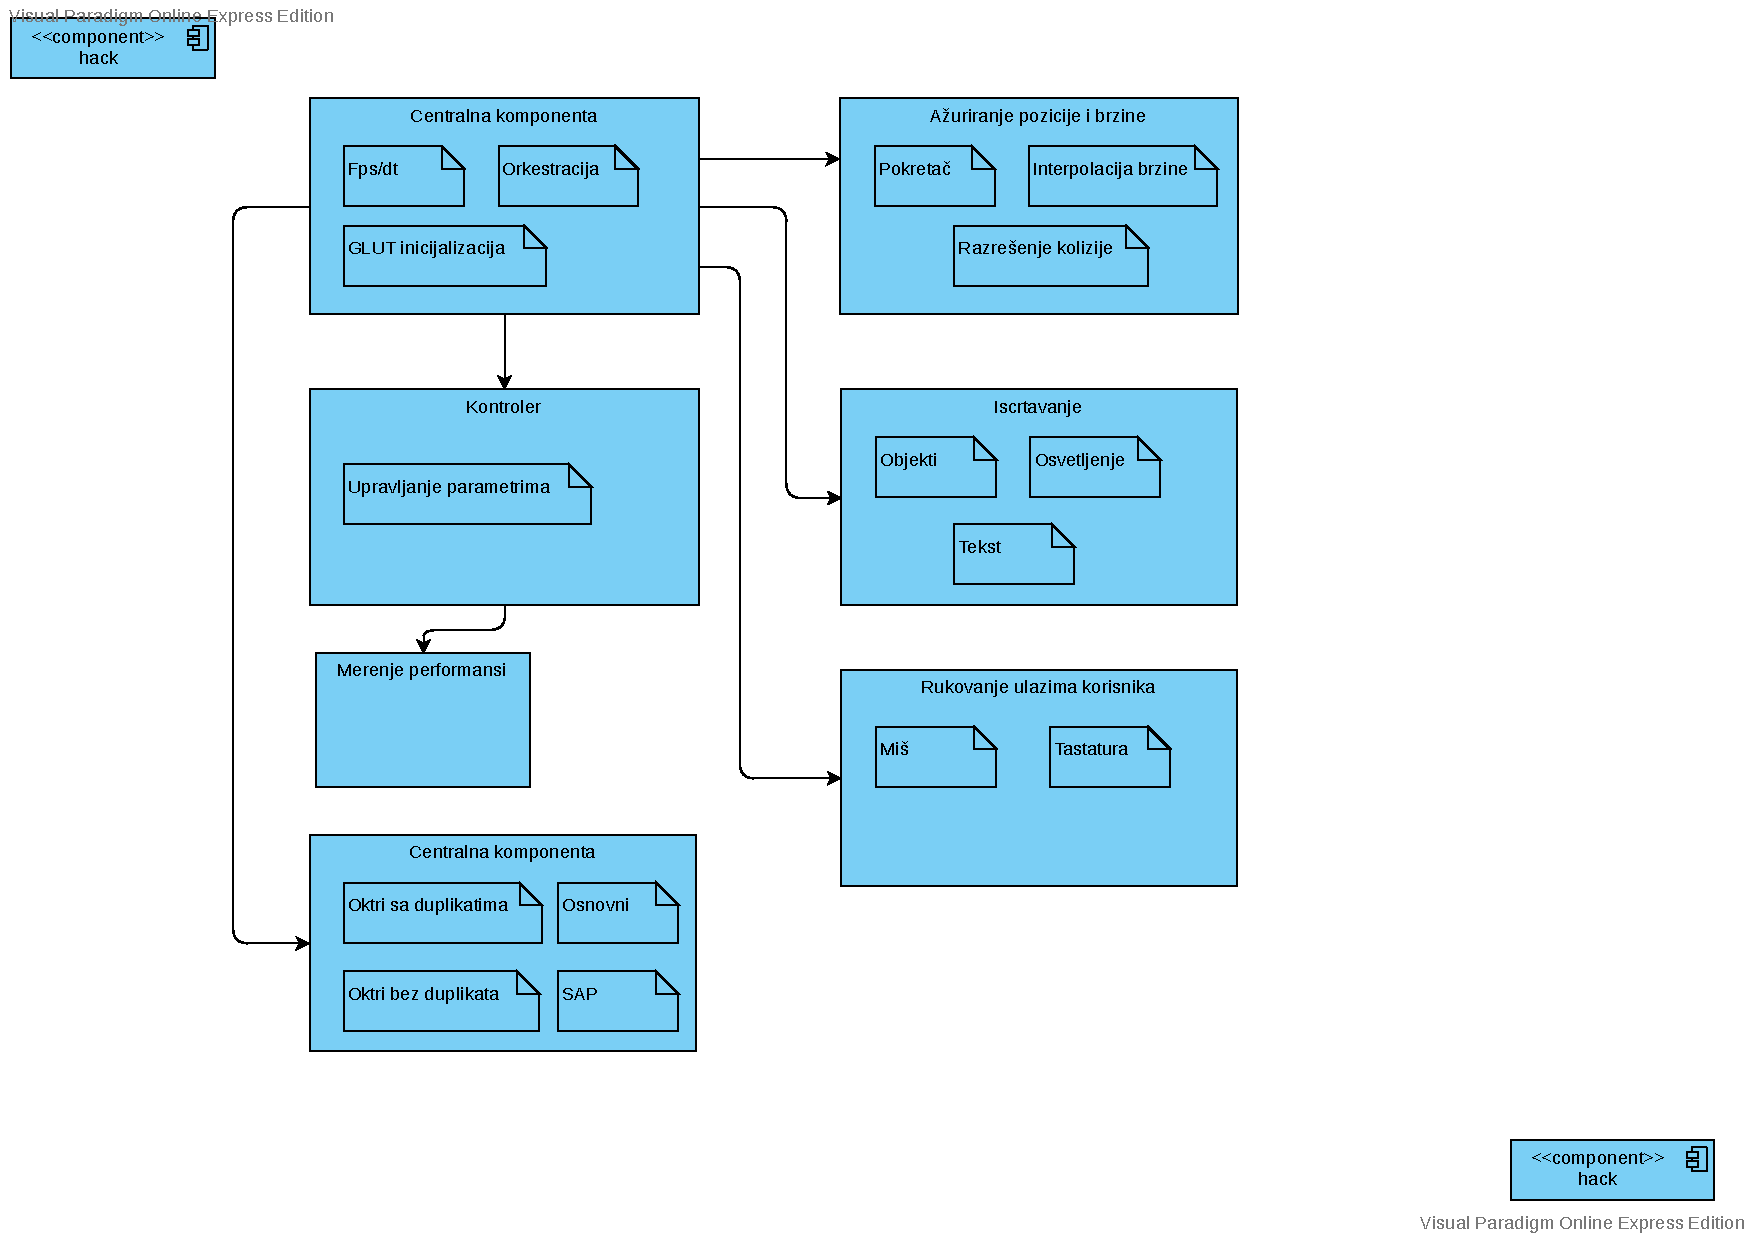
\includegraphics[trim=10 50 100 40,clip,scale=0.9]{archi2.pdf}
	\caption{Arhitektura implementiranog projekta.}
	\label{fig:archi}
\end{figure}

Na slici \ref{fig:archi} je prikazana arhitektura programa sa navedenim komponentama.

\subsection{Kontroler komponenta}

Uloga kontroler komponente je upravljanje parametrima programa i rukovanje njihovim izmenama.
Parametri koji se menjaju kroz kontroler komponentu su: 
\begin{itemize}  
	\item Broj objekata koji su podložni koliziji. 
	Ovo je parametar koji svakako najviše utiče na ponašanje algoritama.
	\item Veličina objekata. 
	Na prvi pogled deluje da vrednost ovog parametra ne utiče previše na performanse, međutim veliki objekti u malom prostoru mogu u velikoj meri da uspore izvršavanje.
	\item Brzina kretanja objekata.
	Ovaj faktor ne utiče na sve algoritme, ali je u slučaju SAP algoritma najbitniji. Može promeniti odlično ponašanje SAP algoritma u slučaju sporog kretanja 
	objekata i učiniti ga algoritmom kvadratne složenosti u najgorem slučaju.
	\item Veličina kontejnera u kome se nalaze i kreću svi objekti. Kontejner je ovde eksplicitno predstavljen, mada bi se inače mogao podrazumevati kao kvadar 
	koji u potpunosti sadrži svet čije se kolizije simuliraju.
	Ovaj parametar daje još jednu perspektivu kako odnos veličine objekata i veličine celog prostora, ovde kontejnera, utiče na performanse.
	\item Maksimalan broj elemenata u listu oktrija.
	Promena maksimalnog broja elemenata u listu pre nego što se on podeli na podoktante utiče "samo" na konstantan faktor vremenske složenosti.
	To uopšte nije zanemarljivo u datom kontekstu i pogodnosti koje daje povoljno izabran parametar su osetne.
	\item Maksimalna dubina oktrija. Veća dubina oktrija je uglavnom povoljnija jer omogućava da se u listovima oktrija nalazi mali broj objekata.
	Međutim, treba biti oprezan ako se može desiti 
	da se veliki broj objekata preklapa unutar jednog oktanta, jer se tada samo gubi vreme i troši dodatna memorija. 
	U tom scenariju pokušavaju se razdvojiti objekti rekurzivnom podelom potprostora, ali pošto se oni presecaju ti pokušaji ne dovode do rezultata.
	\item Da li raditi razrešenje kolizije. 
	Razrešenje kolizije je zaseban problem od problema detekcije kolizije, a pošto se uglavnom koriste oba, onda je dobro videti 
	kako razrešenje kolizije deluje na problem detekcije kolizije u narednim koracima u programu. Pokazuje se da praktično uvek deluje povoljno, pošto onemogućava da se mnogo 
	objekata međusobno preseca, pa se time smanjuje verovatnoća da se stvori veliki klaster objekata koji bi usporio izvršavanje.
	\item Da li je iscrtavanje uključeno ili isključeno. 
	S obzirom na to da je projekat više procesorski nego grafički zahtevan, iscrtavanje uglavnom ne kvari performanse više od 2 do 3 posto.
	Svakako, kada je na sceni više od 30 000 objekata vreme iscrtavanja ima značajniji udeo u ukupnom vremenu izvršavanja,
	pa je za te slučajeve dodata opcija kako bi merenja bila nepristrasna.
	\item Algoritam detekcije kolizije koji se koristi. Podržani su: osnovni (trivijalni) algoritam, oktri sa duplikatima,
	oktri bez duplikata i SAP algoritam. Moguće je i u potpunosti isključiti detekciju kolizije da bi se dobila referentna vrednost vremena izvršavanja.

\end{itemize}  

Kontroler komponenta takođe pruža mogućnost menjanja pravca kretanja objekata. 
Tada svi objekti bivaju usmereni prema trenutnoj poziciji posmatrača. 
Ova funkcionalnost je potrebna pošto ona povećava koncentraciju objekata, 
pogotovo nakon što se odbiju o ivicu kontejnera. Tada će se većina objekata 
naći oko centra kontejnera (kao na slici \ref{fig:ssyank}), što dovodi do eksplozije vremena izvršavanja, posebno u slučaju oktrija sa duplikatima.

\subsection{Komponenta za iscrtavanje}

Sve što se želi prikazati mora se iskazati preko GL funkcija. 
Boja objekata zavisi od osvetljenja i materijala ili teksture koja mu je dodeljena.

Ljudska percepcija boje objekta je zapravo spektar elektromagnetnog zračenja koji se odbija o taj objekat i pada na retinu oka.
U pravom svetu se zraci svetlosti odbijaju od više objekata pre nego što stignu do oka. 
Simulacija takvog ponašanja se naziva praćenje svetlosti (eng. {\em raytracing}).  
Praćenje svetlosti je računarski zahtevno, pa do skoro nije bilo moguće izvršavati ga u realnom vremenu, već samo na farmi servera koji renderuju neku scenu.
2018. godine je firma NVIDIA pustila u prodaju novu seriju grafičkih karti koje hardverski implementiraju praćenje svetlosti. 
U trenutku pisanja ove master teze se ova tehnologija koristi kao hibrid, dakle ne kao zamena već kao dopuna postojećih metoda.

Uobičajeno je da se izvor svetla i materijali objekata opisuju pomoću Fongovog modela senčenja. 
Fongov model je empirijski model osvetljenja. Razvio ga je Bui Tuong Fong i objavio ga u svojoj doktorskoj tezi 1975. godine.
U ovom modelu boja površi se opisuje kao kombinacija difuzne refleksije, tj. odbijanja svetlosti sa grubih površi, 
spekularne refleksije, tj. refleksije sa sjajnih površi, i ambijentalne refleksije, koja predstavlja manju količinu svetlosti 
koja je raspršena kroz celu scenu \cite{Phong}.
OpenGL nudi Fongov model pa se on koristi za opisivanje izvora svetla i materijala svih objekata.


U aplikaciji koja se razvija uključeno je jedno globalno svetlo, a posmatrač može da postavi jos najviše osam svetala na 
proizvoljne statične blokove na mapi. 
Slabljenje svetlosti se izražava preko tri faktora: konstantnog, linearnog i kvadratnog.
Konstantan faktor jednako oslabljuje svetlost svuda, dok linearni i kvadratni faktori oslabljuju svetlost
linearno, odnosno kvadratno, sa rastojanjem od izvora svetlosti.

Ova komponenta se brine i o iscrtavanju teksta, što zahteva nešto više gl poziva nego što bi se očekivalo.

Postavljanje kamere zavisi od pozicije posmatrača i njegovog usmerenja pogleda levo-desno i gore-dole.
Kamera se usmerava od pozicije posmatrača ka pravcu u kome gleda.
Vektor pravca gledanja se dobija prema formuli:

\begin{equation}
\label{eq:camera}
\begin{split}
x = cos(rot_h) \cdot cos(rot_v) \\
y = sin(rot_v) \\
z = cos(rot_h) \cdot  cos(rot_v)	
\end{split}
\end{equation}


\noindent gde je $rot_v$ ugao između $xz$ ravni i pravca gledanja, dok je $rot_h$ ugao rotacije oko $y$ ose.
U OpenGL koordinatnom sistemu je $y$ osa vertikalna, $x$ horizontalna, a $z$ predstavlja dubinu.

\subsection{Centralna komponenta}

Centralna komponenta inicijalizuje GLUT funkcije povratnog poziva, postavlja GL parametre, i pokreće sistem.
Ona definiše i tajmer koji će periodično pozivati ažuriranje sistema i zakazati njegovo ponovno iscrtavanje. 
Ona se takođe stara o računanju vremena između dva uzastopna koraka izvršavanja, redosledu pozivanja funkcija za ažuriranje stanja,
detekcije kolizije, razrešavanja kolizije i iscrtavanja.

\subsection{Komponenta za ažuriranje brzine i pozicije objekata}
% ona radi i razresavanje kolizije

Svakom objektu pridružena je  uređena trojka brojeva u pokretnom zarezu koja označava njegovu poziciju u trodimenzionom prostoru.
Za održavanje pravca kretanja potrebno je čuvati još jednu trojku vrednosti koja predstavlja vektor brzine kretanja.
Ako se pritom želi da objekat postepeno ubrzava kada se na njega primeni sila, ili da postepeno usporava 
kada prestane delovanje sile, onda se uz pomenute podatke mora čuvati još jedna trojka brojeva, koja predstavlja ciljnu brzinu.
Postepeno ubrzavanje se koristi pri kretanju posmatrača. 
Kada se pritisne dugme na tastaturi za pomeranje posmatrača, očekivano ponašanje je da posmatrač neće istog trenutka 
početi da se kreće maksimalnom brzinom, već da će postepeno ubrzavati.
Slično, kada se ovo dugme pusti, "sila" koja je delovala na posmatrača je nestala, ali je on imao momenat pa će
nastaviti da se kreće još malo unapred.

Potrebno je pažljivo razmotriti kako posmatrač treba da se kreće na komandu da ide napred-nazad ili levo-desno.
Naivno razmišljanje bi navelo na ideju da je prilikom kretanja levo-desno potrebno povećati ili smanjiti vrednost pozicije $x$ koordinate posmatrača,
odnosno da se menja $z$ koordinata posmatrača kada treba da se kreće napred-nazad.
To ipak nije dobro rešenje pošto kada neko želi da se pomeri on ne razmišlja apsolutno, u terminima strana sveta, na koju će stranu, 
već relativno u odnosu na njegovo trenutno usmerenje (dato formulom \ref{eq:camera}).
Neka je dat trodimenzioni jedinični vektor $v$ koji predstavlja usmerenje pogleda; tada je vektor 
kretanja unapred jednak: 
$$ v_{napred} = \frac{(v_x, 0, v_z)^T}{\|(v_x, 0, v_z)^T\|} $$
Vektor kretanja unapred ima nulu za vrednost $y$ koordinate pošto usmerenje pogleda gore-dole ne utiče na pravac kretanja.
Pritom se vektor normira kako se ne bi sporije kretalo u slučaju gledanja gore ili dole, 
pošto su tada vrednosti $v_x$ i $v_z$ male.
Slično, vektor kretanja u stranu se računa po formuli:
$$ v_{bok} = \frac{(-v_z, 0, v_x)^T}{\|(-v_z, 0, v_x)^T\|} $$

Vrednosti prve i treće koordinate vektora su zamenjene iz razloga što kada se gleda pravo u smeru $x$ ose, 
onda je bočno kretanje duž $z$ ose. Razlog za promenu znaka uz $v_z$ se ogleda u orijentaciji $z$ ose u odnosu na $xz$ ravan.
Koordinatni sistem koji se koristi je prikazan na slici \ref{fig:coord}.

\begin{figure}[h!]
	\centerfloat
	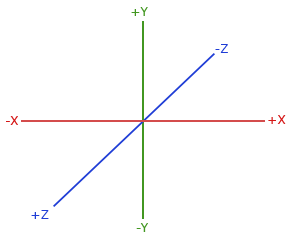
\includegraphics[scale=0.75]{coord.png}
	\caption{OpenGL koordinatni sistem.}
	\label{fig:coord}
\end{figure}

Kontejner koji sadrži objekte koji se sudaraju se stara o njihovom pravilnom odbijanju o ivice ograničavajućeg prostora.
Kada se objekat sudari sa ivicom kontejnera onda je potrebno reflektovati onu koordinatu vektora
brzine objekta koja odgovara osi duž koje su se sudarili.
Objekti će nekada delom izaći van kontejnera, pa se tada oni pomeraju u unutrašnjost tako da jedna njihova strana bude uz stranu kontejnera.

Kada se, na primer, na kuglu koja stoji uz zid primeni sila koja nije upravna na stranu zida, onda kugla neće ostati nepokretna,
već se kretati paralelno uz stranu zida. Isti princip važi i za kretanje posmatrača uz zid jer je 
takvo ponašanje standardno za sve video igre.

Detekcija kolizije kao rezultat daje parove svih objekata u koliziji. 
Na te parove se primenjuje algoritam za razrešenje kolizije prema formulama (\ref{eq:mtv}) i (\ref{eq:razresenje}).

\subsection{Komponenta za merenje performansi}
\label{sec:perf}

Ova komponenta služi za prikupljanje podataka kako bi se uradila evaluacija data u poglavlju \ref{sec:evaluacija}.
Jedna instanca merenja predstavlja jedan korak izvršavanja i sastoji se od 
vremena izvršavanja koraka, veličine objekta, broja objekata i dodatnih podataka u zavisnosti od toga 
koji algoritam detekcije kolizije se koristi. 
Sakupljeni podaci se ne zapisuju direktno u izlaznu datoteku, pošto bi 
to usporavalo izvršavanje, već se čuvaju u vektoru, 
i tek kada je gotovo celokupno merenje, vrši se ispis u odgovarajuću datoteku.

\subsection{Komponenta za rukovanje ulazima korisnika}

Komponenta za rukovanje ulazima korisnika definiše funkcije povratnog poziva koje će FreeGLUT pozivati.
Od funkcija biće potrebne funkcija za akciju pritiska dugmeta tastature, puštanje dugmeta, kao i 
radnja koja se vrši dok je dugme pritisnuto. 
Za poslednju navedenu akciju se za svako dugme sa tastature mora ručno implementirati pamćenje stanja pritisnutosti.
Ako se želi akcija na pritisak specijalnih dugmeta  
poput F1, F5, strelice i slično, onda se zahteva definisanje odvojenih funkcija za njih.

Što se tiče reakcija na pritisnuto dugme, prva ideja je da se direktno pozove odgovarajuća akcija. 
To je u redu ako je ta akcija na primer izlazak iz programa, promena izabranog algoritma, ili neka druga jedinična akcija.
Ako je pak u pitanju akcija poput kretanja napred, onda bi takvo ponašanje imalo neprijatan efekat. 
Oslanjalo bi se na učestale ponovljene signale da je dugme pritisnuto, koji u praksi uopšte nisu periodični.
To bi dovelo do efekta "seckanja" prilikom kretanja i brzina kretanja bi zavisila od mogućnosti glavne petlje događaja da signal pritiska dugmeta često i ravnomerno poziva.
Takođe, mogla bi se desiti  dva uzastopna signala pritiska dugmeta za kretanje napred između dva iscrtavanja scene. 
Da li bi tada trebalo da se napravi duplo veći pomeraj?
Ispravan odgovor bio bi ne, ali bi to bio efekat ovakve implementacije.

Ispravno rešenje bilo bi da se zapamti da je dugme pritisnuto,  a da se na ovaj događaj reaguje  tek zajedno sa ostalim ažuriranjima 
stanja i pozicija, što se dešava periodičnim pozivima komponente koja je za to zadužena. Tako je reakcija nezavisna od učestalosti 
slanja ponovnih signala da je dugme pritisnuto, štaviše, oni su sada nepotrebni. 

Što se tiče događaja miša, postoje tri funkcije koje je potrebno implementirati. Prva se odnosi na događaj pritiska 
dugmeta miša, druga na pomeraj miša, dok se treća tiče događaja pomeranja miša dok je neko dugme na njemu pritisnuto.
Potrebno je pratiti vrednost svakog pomeraja miša i na osnovu toga izračunati novu horizontalnu i vertikalnu rotaciju 
kamere, odnosno posmatračevog usmerenja.
Kako kursor miša ne bi napustio prozor programa, 
potrebno ga je nakon svakog pomeraja vratiti u centar prozora.
Kursor miša se podrazumevano ne prikazuje na ekranu, a dodata je opcija da se prikaže i da dobije nazad slobodu da napusti prozor.

\subsection{Komponenta za detekciju kolizije}

S obzirom na tematiku ovog rada, najznačajnija i najinteresantnija je funkcionalnost koju pruža ova komponenta.
Algoritmi za detekciju kolizije su implementirani u odvojenim klasama, ali imaju isti interfejs.
Svaka klasa implementira metodu kojoj se prosleđuje vektor objekata za koje treba proveriti da li su u koliziji
i vraća sve parove objekata koji jesu u koliziji. Takođe, svaka klasa implementira metod koji daje relevantne podatke 
o stanju algoritma specifičnom za njega (npr. broj elemenata u unutrašnjim čvorovima oktrija ili broj 
zamena u SAP algoritmu). Oni se koriste za merenje i za ispisivanje trenutnih informacija prilikom testiranja.

\section{Vizuelizacija}

U ovoj sekciji biće predstavljen izgled razvijene aplikacije. 
Izvorni kod implementacije je dostupan na \url{https://github.com/kredenac/collision-detection}.
Program je namenjen za interaktivno korišćenje. 
Korisnik može da se kreće, pomera kameru (usmerenje pogleda), menja parametre koji utiču na detekciju kolizije,
zapaža rezultate posmatranjem objekata na sceni, posmatranjem prikazanih vrednosti ili izvršavanjem odgovarajućih merenja
(zapisivanjem informacija o svakom koraku izvršavanja).

Na slici \ref{fig:ssdefault} prikazano je podrazumevano stanje programa prilikom njegovog pokretanja.
U donjem levom uglu su ispisane relevantne informacije, od kojih su najbitnije broj objekata 
i broj slika u sekundi. Takođe je prikazan algoritam koji se koristi, parametri specifični za njega, kao 
i veličina objekta, brzina kretanja (kada nije izabrana podrazumevana vrednost),  da li je uključeno razrešavanje kolizije ili ne  i
broj objekata koji su u koliziji.

\begin{figure}[h!]
	\centerfloat
	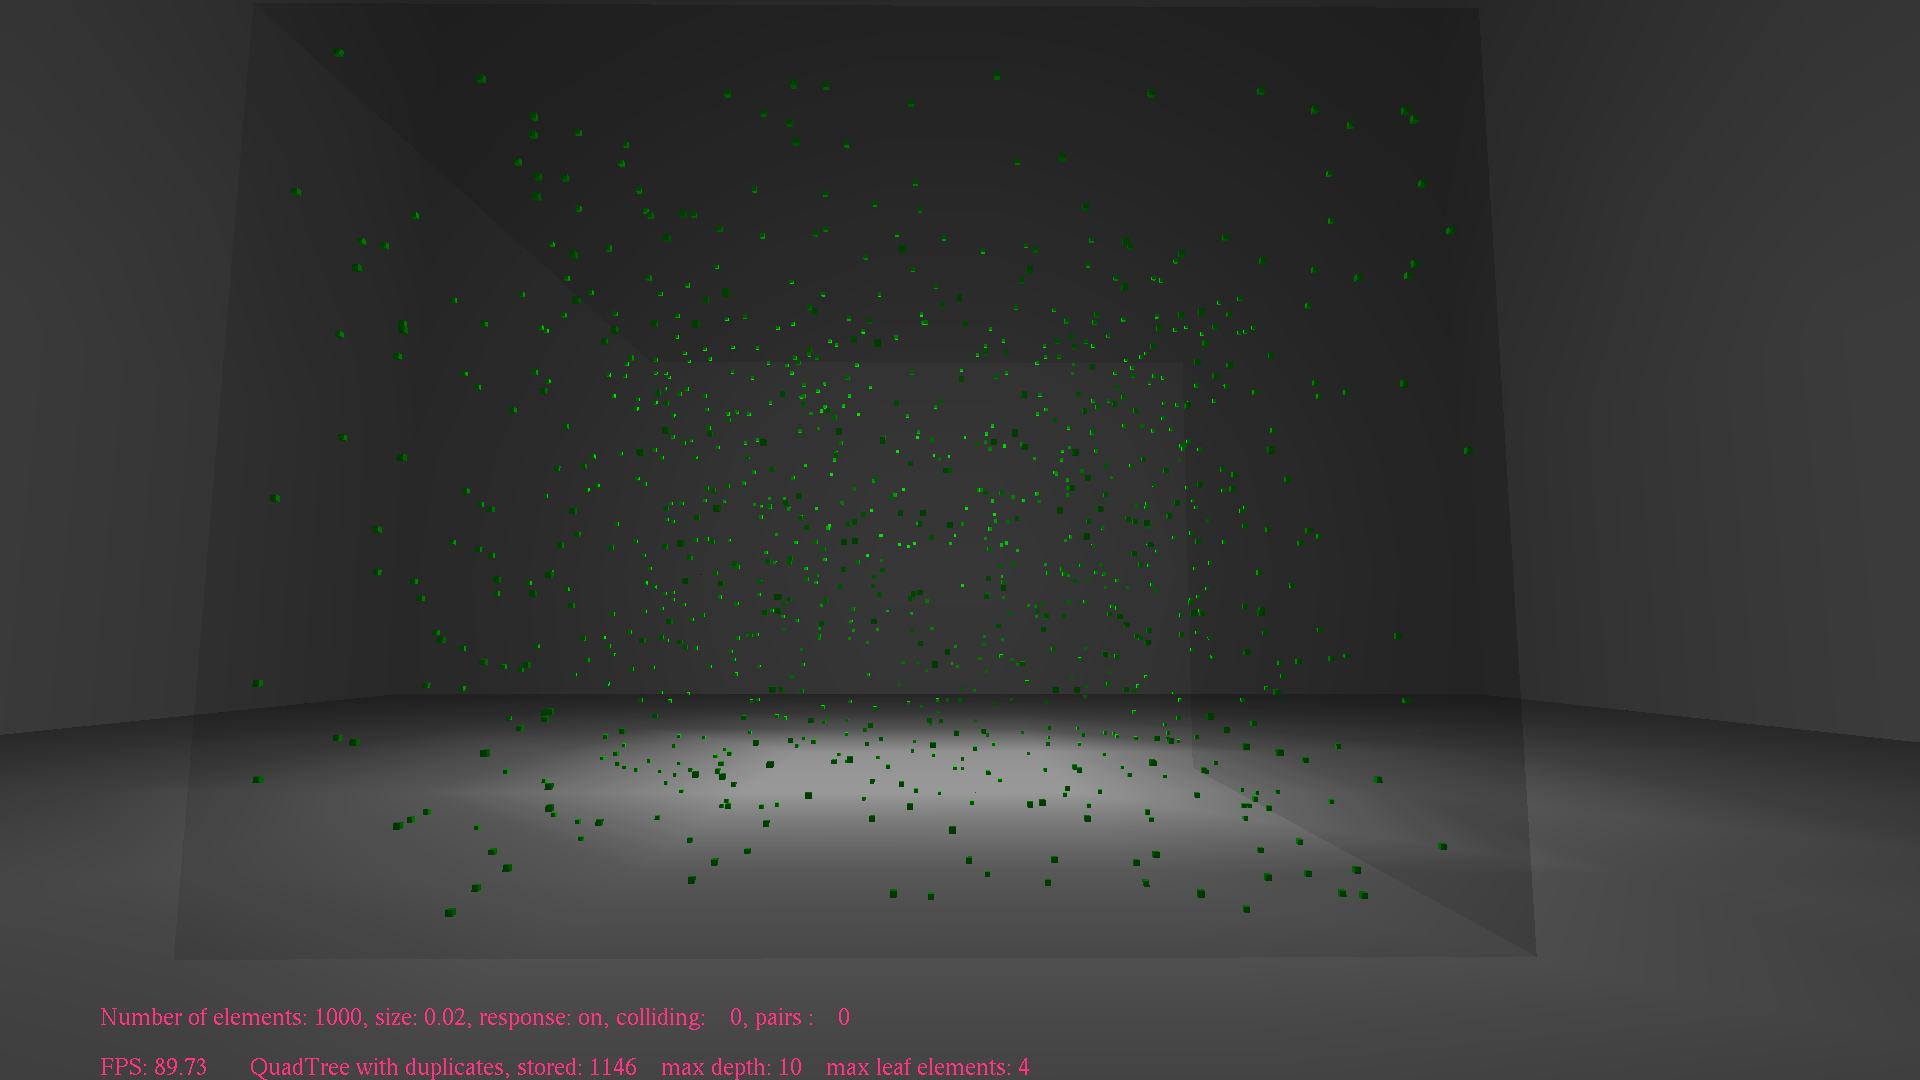
\includegraphics[scale=0.3]{ssdefault.png}
	\caption{Snimak ekrana - podrazumevano stanje programa.}
	\label{fig:ssdefault}
\end{figure}

\noindent Desnim klikom miša mogu se prikazati 
na levoj strani ekrana kontrole,
poput one kojom je moguće povećati kontejner ili broj objekata, kao na slici \ref{fig:ssinfo}.

\begin{figure}[h!]
	\centerfloat
	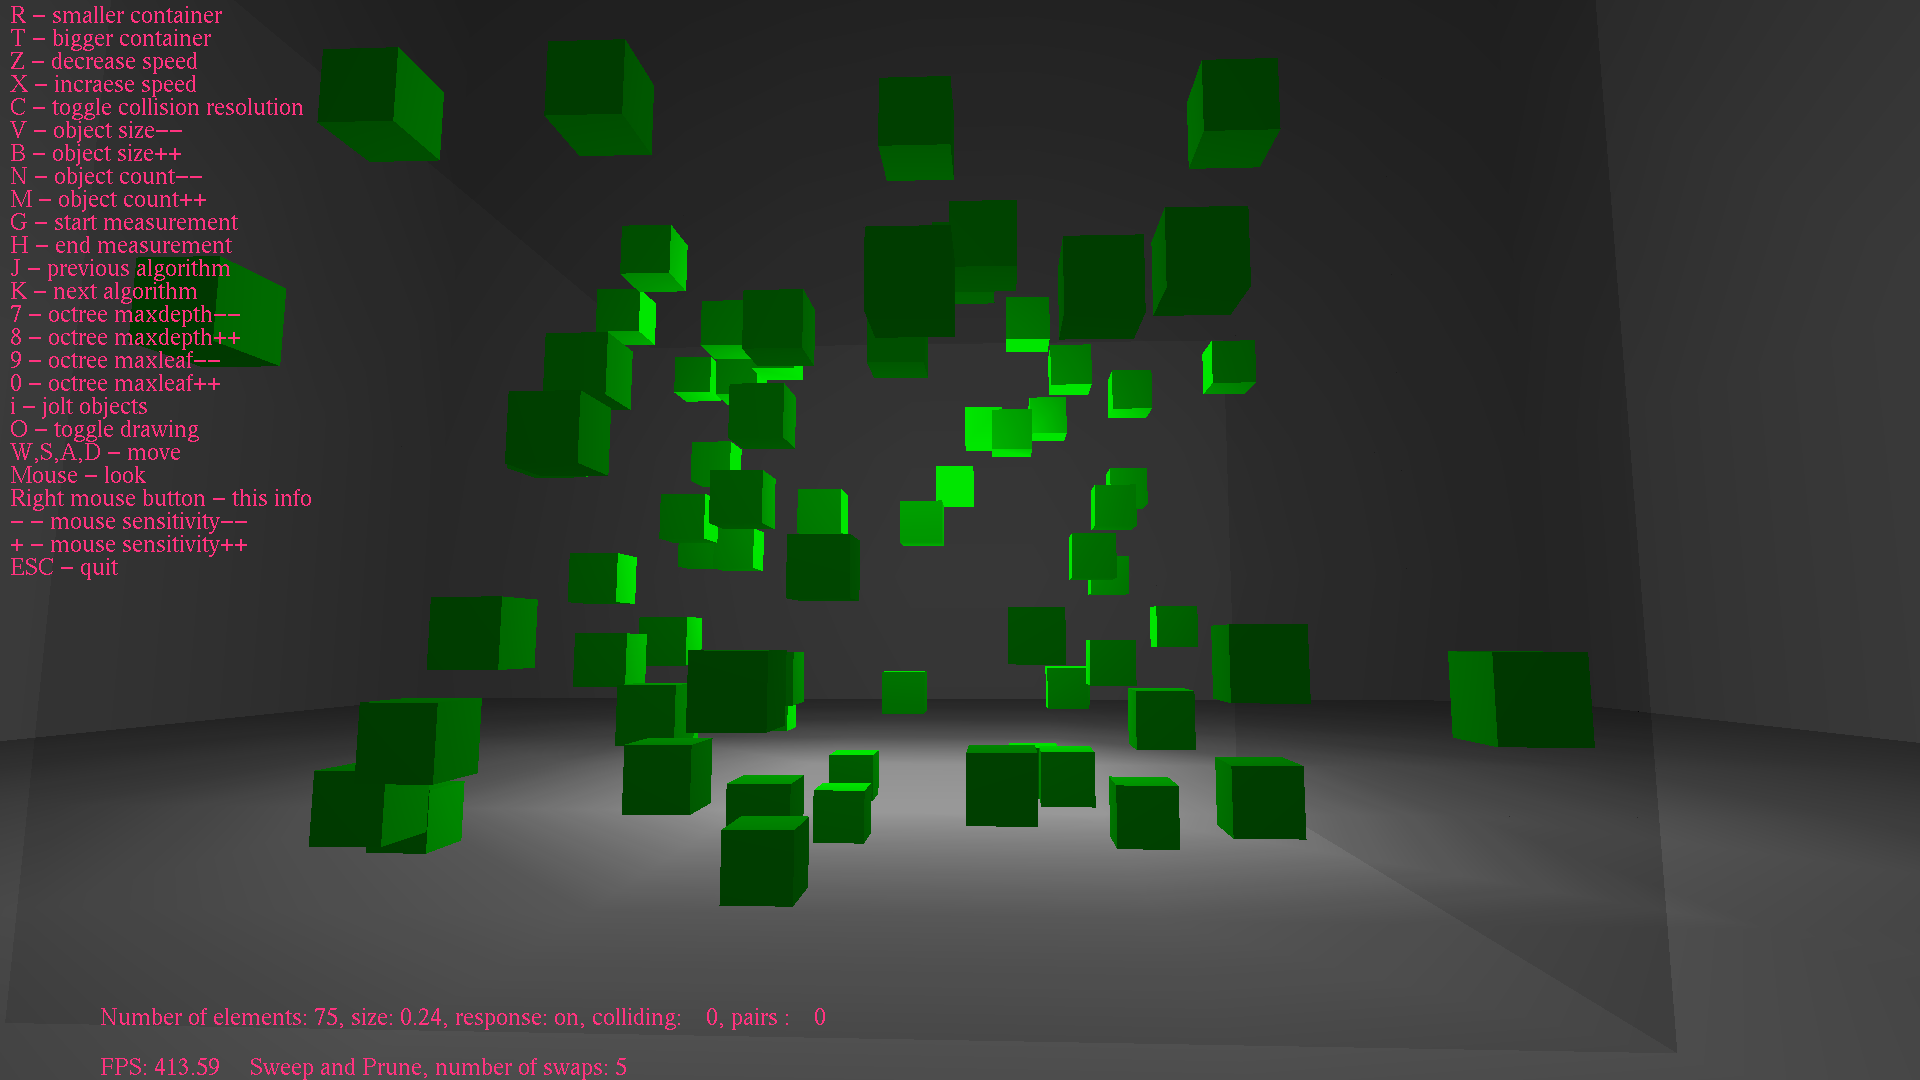
\includegraphics[scale=0.3]{ssinfo.png}
	\caption{Snimak ekrana - prikazane kontrole.}
	\label{fig:ssinfo}
\end{figure}

\noindent Na slici \ref{fig:ssyank} je prikazana situacija kada postoji grupa objekata u centru kontejnera i takav slučaj biće 
razmatran u evaluaciji (glava \ref{sec:evaluacija}).

\begin{figure}[h!]
	\centerfloat
	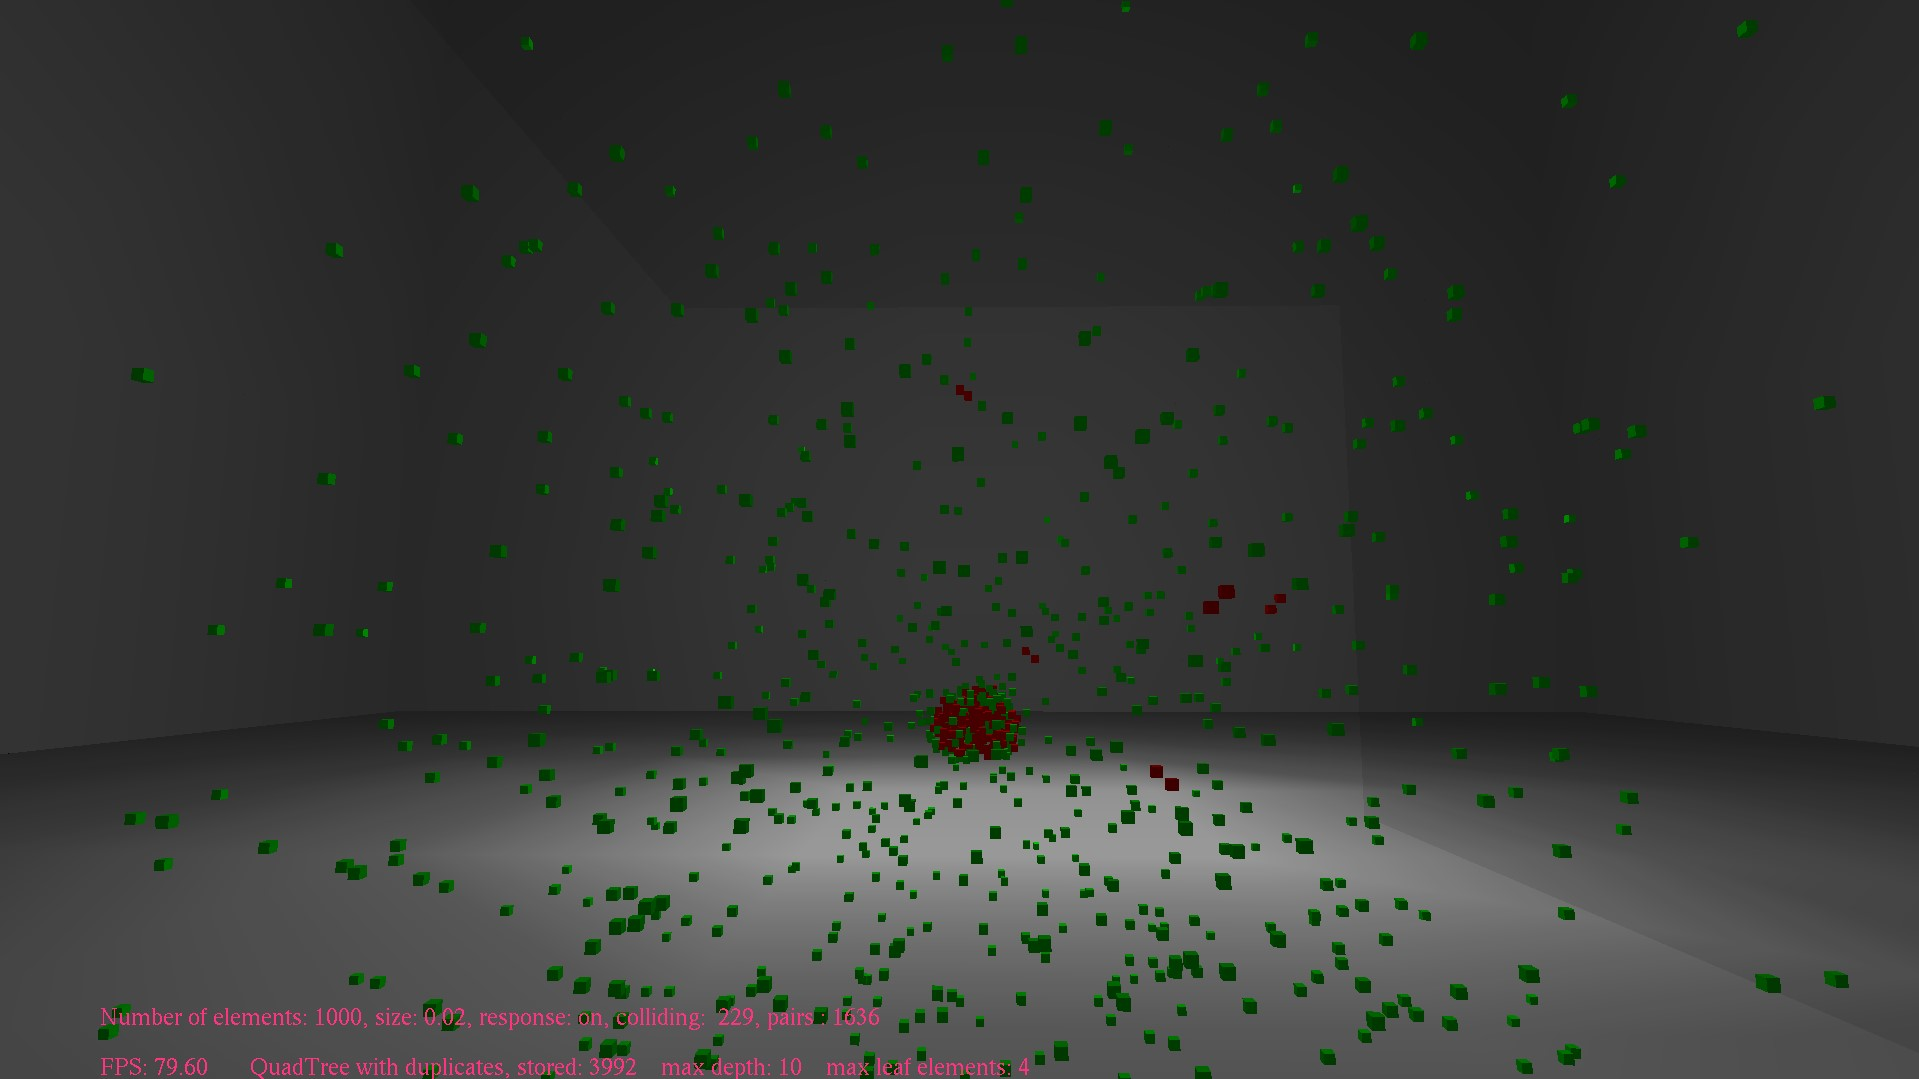
\includegraphics[scale=0.3]{ssyank.jpg}
	\caption{Snimak ekrana - klaster objekata u centru.}
	\label{fig:ssyank}
\end{figure}

% ==============================================================================
\chapter{Evaluacija}
\label{sec:evaluacija}
% ==============================================================================

U ovom poglavlju biće izloženi rezultati merenja vremena izvršavanja koraka simulacije.
Da bi se dobile sve vrednosti $dt$ koje predstavljaju proteklo vreme između dva uzastopna ažuriranja scene
koristi se komponenta za merenje performansi opisana u delu \ref{sec:perf}, a za dobijanje precizne vrednosti trenutnog vremena se koristi funkcija iz GLUT biblioteke.
U daljem tekstu se pod terminom "relativan $dt$" podrazumeva vrednost:
$$ \frac{ dt }{16.67} $$

Razlog za deljenje brojem 16.67 je taj što je poželjan minimalan broj iscrtavanja u sekundi 60, 
što je $1/60$ sekunde, odnosno 16.67 milisekundi u terminima proteklog vremena $dt$.
Tako relativan $dt$ predstavlja umnoške od 16.67 milisekundi i lakše se interpretira
(npr. mere 33.33 i 8.33 milisekundi redom postaju 2 i 0.5 relativnog $dt$).

Sva merenja su izvršena na računaru sa sledećom konfiguracijom:
\begin{itemize}  
	\item Procesor - Intel Core i5-6600K 
	\item Grafička karta - NVIDIA GeForce GTX 1060 WINDFORCE OC 6G
	\item RAM memorija - Kingston HyperX FURY 8GB 2133MHz DDR4 
	\item Matična ploča - ASUS Z170-A
\end{itemize}  
Pritom se vodilo računa da nisu pokrenuti drugi programi koji bi uticali na rezultate.
Procesorski takt je postavljen na 4.4 GHz.

Za pretprocesiranje i prikaz podataka korišćen je programski jezik Python,
biblioteka pandas za obradu podataka i biblioteka matplotlib
za pravljenje grafika.

\section{Opšti zaključci}

Za početak, potrebno je ustanoviti  koliki uticaj na vreme izvršavanja ima postupak iscrtavanja.
U slučaju da iscrtavanje troši veći ili sličan udeo vremena  u odnosu na detekciju kolizije bilo bi nepravilno meriti ih zajedno.
Kao što je već pomenuto, u programu je omogućeno isključiti iscrtavanje.

Na svim narednim graficima (osim \ref{fig:dtSapCrawl}) prikazane su sledeće referentne vrednosti:
\begin{itemize}  
	\item Prava koja predstavlja linearnu zavisnost $y$ od $x$ (prikazana isprekidanom zelenom bojom).
	Koeficijent prave je jednak odnosu najmanje $y$ i najmanje $x$ vrednosti, tj. $y_0/x_0$.
	\item Ciljna vrednost od 60 slika po sekundi (prikazana žutom bojom).
	60 slika po sekundi je traženi minimum za računare.
	\item Ciljna vrednost od 30 slika po sekundi (prikazana crvenom bojom).
	30 slika po sekundi je traženi minimum za igre na konzolama.
\end{itemize}  

\begin{figure}[h!]
	\centerfloat
	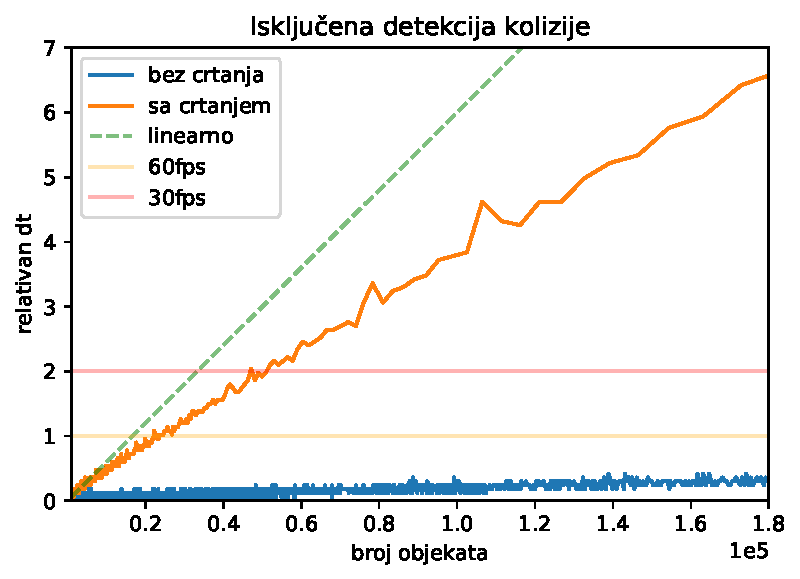
\includegraphics[
		trim= 0 0 0 19, clip,
		scale=1]{idleDrawVsNoDraw.pdf}
	\caption{Relativan $dt$ u zavisnosti od broja objekata u slučaju kada je isključena detekcija kolizije.}
	\label{fig:drawVsNoDraw}
\end{figure}

Na slici \ref{fig:drawVsNoDraw} prikazan je grafik zavisnosti relativnog $dt$ od broja objekata.
Detekcija kolizije je isključena, tako da na vreme utiče samo kretanje objekata i iscrtavanje.
Kada je iscrtavanje uključeno onda vreme izvršavanja raste linearno (sa koeficijentom manjim od 1).
Na oko 24 000 objekata vrednost relativnog $dt$ prelazi 1, a na 50 000 objekata ona prelazi 2. 
Sa druge strane, kada je crtanje isključeno vreme izvršavanja je mnogo manje. 
Ono i dalje raste linearno sa brojem objekata, ali je konstanta uz linearni član za red veličine manja nego kada je iscrtavanje uključeno.
Čak i kada je broj objekata veći od 180 000 program se izvršava sa malim relativnim $dt$, 
što znači da je to vreme zanemarljivo u odnosu na vreme potrebno za detekciju kolizije.

Na slici \ref{fig:basic} prikazana je zavisnost relativnog $dt$ od broja objekata kada se koristi 
trivijalan algoritam za detekciju kolizije. Na grafiku se uočava nagli rast, što je i očekivano pošto 
je algoritam kvadratne vremenske složenosti.
Čak i za manje od 2000 objekata relativan $dt$ postaje veći od 1, 
a na 2500 veći od 2. Takvo rešenje je neupotrebljivo za veći broj objekata. Jedina "prednost" je što 
je vreme izvršavanja isto koliko god se brzo objekti kretali, koje god da su veličine i koliko god 
da ih se međusobno preseca.

\begin{figure}[h!]
	\centerfloat
	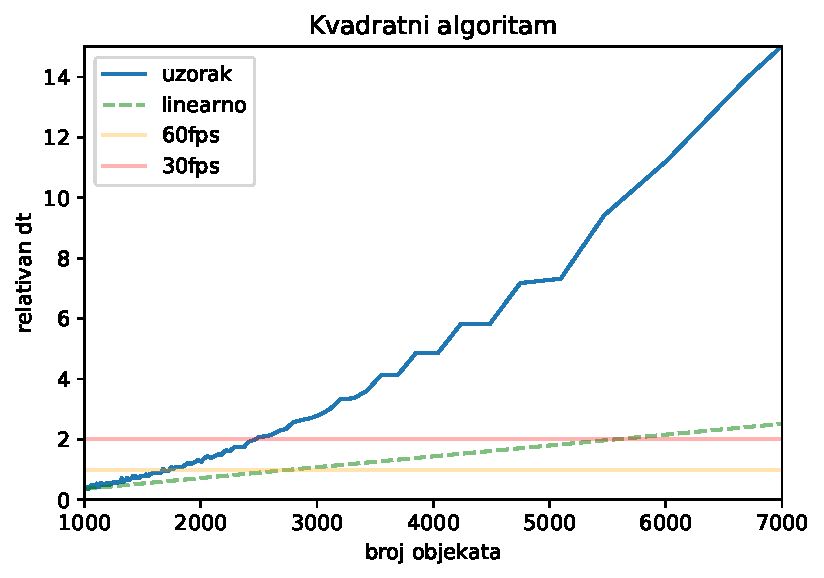
\includegraphics[
		trim= 0 0 0 19, clip,
		scale=1]{basicCollision.pdf}
	\caption{Relativan $dt$ u zavisnosti od broja objekata - trivijalan algoritam.}
	\label{fig:basic} 
\end{figure}

\section{Oktri}

Na slici \ref{fig:oktri1} su prikazane performanse oktrija sa maksimalnom dubinom od deset nivoa i sa maksimalnom vrednošću od četiri elementa u listu.
Može se primetiti da on za manji broj objekata prati referentnu liniju linearne zavisnosti.
Kada je broj objekata mali, on je višestruko bolji od prethodno prikazanog (trivijalnog) algoritma.
Broj slika u sekundi pri korišćenju oktrija pada ispod 60fps tek nakon 12 000 objekata, a ispod 30fps nakon 20 000 objekata.
I za manji broj objekata je višestruko bolji u odnosu na prethodno prikazani,
pada ispod 60fps tek nakon 12 000 objekata, i ispod 30fps nakon 20 000.
Ipak, na slici \ref{fig:oktri2} prikazano je ponašanje istog algoritma za veće vrednosti broja objekata. 
Može se uočiti brže udaljavanje od referentne prave linearne zavisnosti,
što je i očekivano, s obzirom na to da algoritam nije linearne vremenske složenosti.

\begin{figure}[h!]
	\centerfloat
	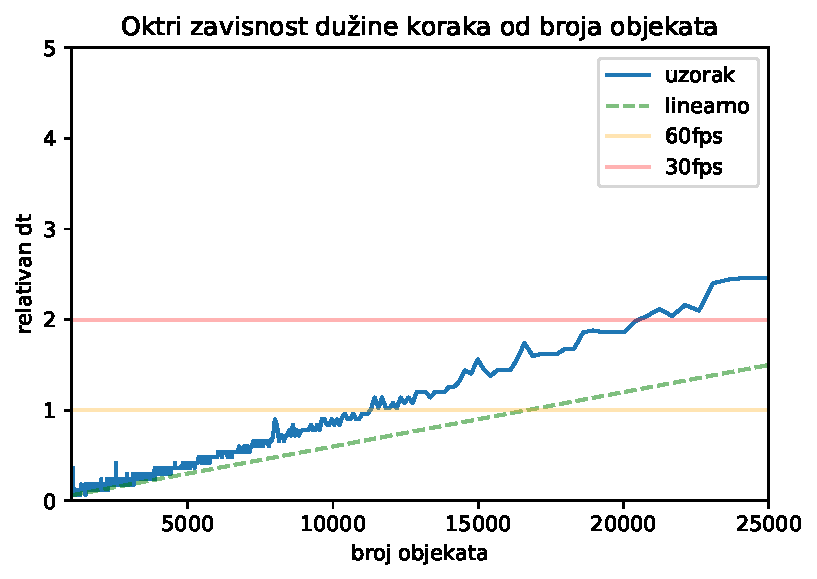
\includegraphics[
		trim=0 0 0 19,clip,
		scale=1]{oktri_dt_vs_numobj.pdf}
	\caption{Zavisnost relativnog $dt$ od broja objekata - oktri.}
	\label{fig:oktri1}
\end{figure}

\begin{figure}[h!]
	\centerfloat
	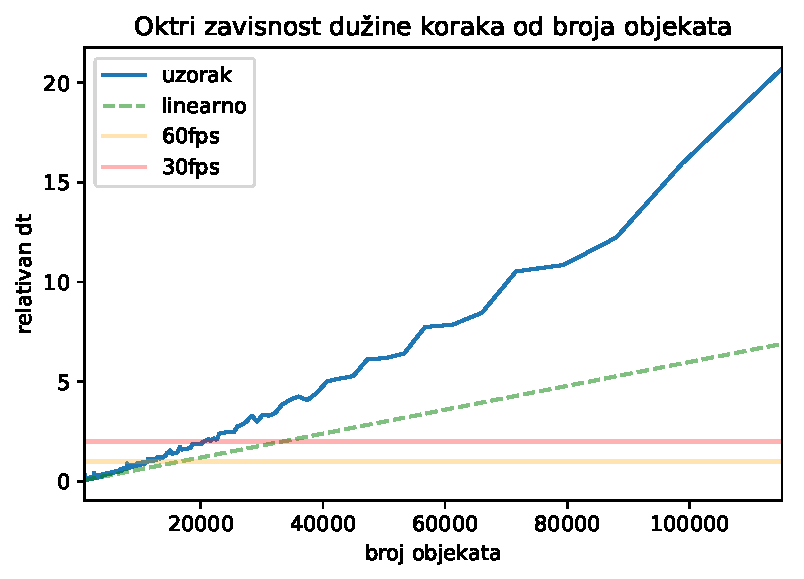
\includegraphics[
		trim=0 0 0 19,clip,
		scale=1]{oktri_dt_vs_numobj_zoomout.pdf}
	\caption{Zavisnost relativnog $dt$ od broja objekata za veći broj objekata - oktri.}
	\label{fig:oktri2}
\end{figure}

Grafici \ref{fig:oktri1} i \ref{fig:oktri2} se odnose na oktri sa duplikatima.
Oktri sa i bez duplikata imaju slične performanse dok je broj objekata ispod 5000.
Kao što se vidi na slici \ref{fig:dupvsnodup}, vreme izvršavanja u zavisnosti od broja objekata kod oktrija bez duplikata raste brže od oktrija sa duplikatima.

\begin{figure}[h!]
	\centerfloat
	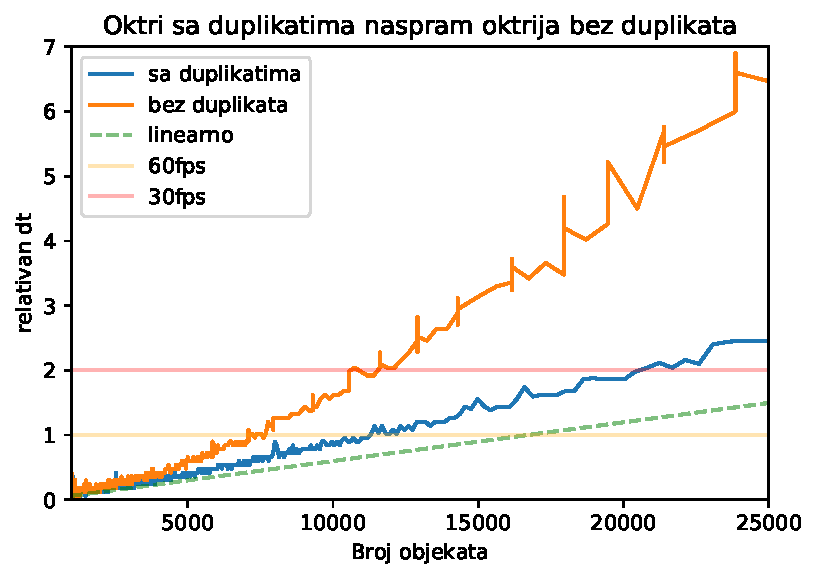
\includegraphics[
		trim=0 0 0 19,clip,
		scale=1]{octree_dup_vs_nodup.pdf}
	\caption{Zavisnost relativnog $dt$ od broja objekata za veći broj objekata - oktri sa duplikatima naspram oktrija bez duplikata.}
	\label{fig:dupvsnodup}
\end{figure}

Međutim, postoje situacije kada oktri bez duplikata ima bolje performanse. 
Jedna od njih je kada se veliki broj objekata nalazi na istom mestu, kao što je slučaj na slici \ref{fig:ssyank}.
Za potrebe demonstriranja ove pojave se koristi scenario gde se objekti nasumično kreću i onda svi bivaju povučeni ka jednoj istoj tački.
Tada se svi nalaze na istom mestu za trenutak, i potom se razilaze.
Ovaj efekat prikazan je na slici \ref{fig:octreSpike} i mogu se uočiti i tri manja skoka za oktri bez duplikata (prikazana plavom bojom),
i dva skoka reda veličine za oktri sa duplikatima (prikazana narandžastom bojom).
Za potrebe ovog merenja je isključeno razrešenje kolizije da bi više objekata bilo u koliziji, što pokazuje interesantno svojstvo da iako je za razrešavanje kolizija potrebna dodatna obrada, 
ona onemogućava grupisanje preseka objekata i time ubrzava izvršavanje algoritma zasnovanog na oktrima (i mnogih drugih algoritama detekcije kolizije).


\begin{figure}[h!]
	\centerfloat
	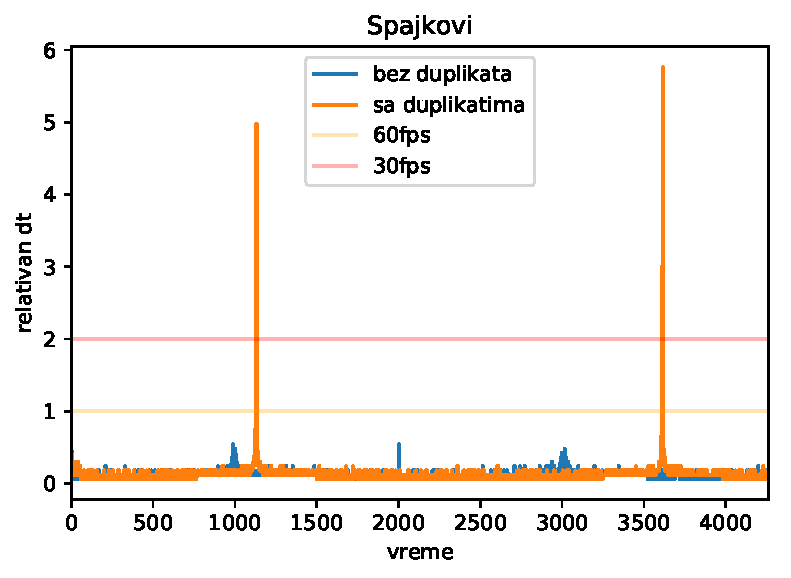
\includegraphics[
		trim=0 0 0 19,clip,
		scale=1]{octreeSpikes.pdf}
	\caption{Usporenje oktrija pri klasterovanju objekata. Pikovi su trenuci kada su objekti klasterovani. }
	\label{fig:octreSpike}
\end{figure}


Tokom razvoja projekta kao vrednost maksimalnog dozvoljenog broja elemenata u listu bila je odabrana konstanta 4. 
Ova vrednost je izabrana vodeći se logikom da je manja vrednost pogodna zbog izbegavanja kvadratnog broja upoređivanja, 
a da nije dobro ni da je sasvim mala, jer bi se listovi previše često delili. 
Na slici \ref{fig:octree_leaf} se zapaža da ovako odabrana vrednost nije loš izbor i tada je broj slika u sekundi 69 (0.89 relativan $dt$). 
Ispostavlja se da 1 predstavlja najlošiju vrednost za ovaj parametar pošto dovodi do viška rekurzivnog particionisanja prostora.
Pokazuje se, takođe, da sa porastom vrednosti maksimalnog broja elemenata u listu relativan $dt$ opada sve do vrednosti 32, od koje počinje da raste.
Najbolje performanse algoritam postiže za vrednost 32, kada je broj slika u sekundi 94 što je čak za 36.2\% bolje (u odnosu na prethodnih 69fps)! 
Ubrzanje od 36.2\% je u praksi veoma značajno, pogotovo što je postignuto promenom samo jednog koeficijenta.
U svim ovim merenjima broj objekata je fiksan i iznosi 10 000 objekata i korišćen je oktri sa duplikatima.

\begin{figure}[h!]
	\centerfloat
	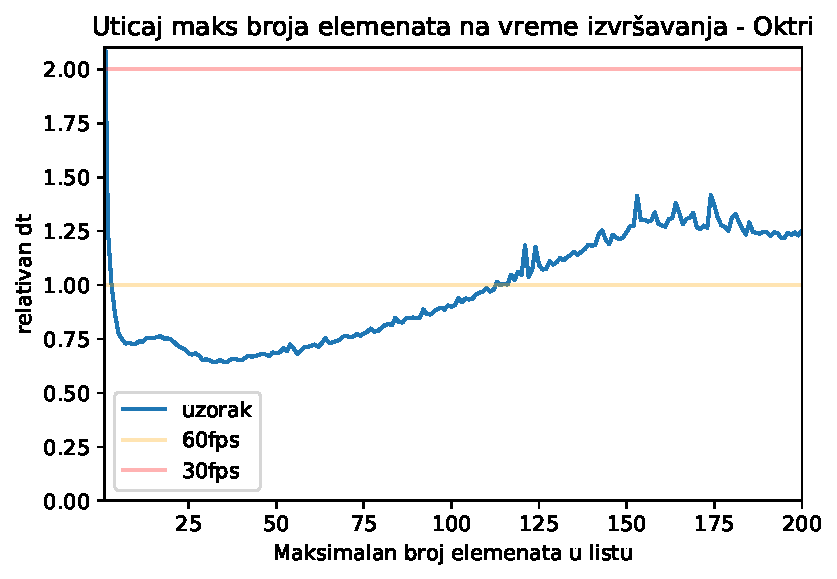
\includegraphics[
		trim=0 0 0 19,clip,
		scale=1]{octree_leaf.pdf}
	\caption{Relativan $dt$ u zavisnosti od maksimalnog broja elemenata u listu oktrija}
	\label{fig:octree_leaf}
\end{figure}


Maksimalna dubina oktrija je postavljena na 10 tokom razvoja projekta. 
Njenom promenom se ne postiže mnogo, osim jakog usporenja kad bi se postavila na 1 ili 2, jer se tad skoro svi parovi objekata moraju ispitati.
Vrednosti 9 do 12 predstavljaju segment pogodnih vrednosti za odabir maksimalne dubine, jer omogućavaju dovoljno particionisanje prostora 
da se izbegne kvadratan broj operacija ispitivanja preseka,
a u slučaju da se više objekata preklapa izvršiće rano zaustavljanje rekurzivnih podela koje pokušavaju da ih razmeste u više oktanata.

\section{SAP}


Algoritam SAP pokazuje dobro ponašanje dok je broj objekata ispod 11 000 (slika \ref{fig:sap1}).

\begin{figure}[h!]
	\centerfloat
	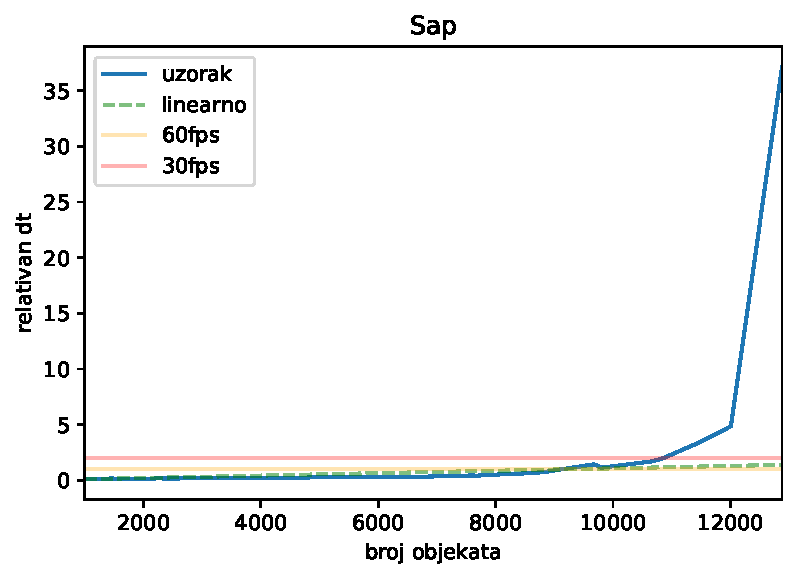
\includegraphics[
		trim=0 0 0 19,clip,
		scale=1]{sap1.pdf}
	\caption{Zavisnost relativnog $dt$ od broja objekata - SAP.}
	\label{fig:sap1}
\end{figure}

Kada je broj objekata veći od 11 000 počinje da se manifestuje njegova glavna razlika u odnosu na ostale algoritme.
Naime, za veći broj objekata potrebno je više vremena da se obradi detekcija kolizije, što produžava vreme između dva ažuriranja pozicija.
Što je vreme između dva ažuriranja pozicija veće, to je i više vremena proteklo u simulaciji, samim tim će i objekti biti udaljeniji od svojih prethodnih pozicija 
nego što bi bio slučaj da je proteklo vreme između dva koraka kraće.
Veći pomeraj objekata znači da je niz koji se održava sortiranim u SAP algoritmu daleko od toga da bude 
sortiran, pa je potrebno izvesti dodatne zamene elemenata u nizu da bi on ponovo postao sortiran. 
Time se iznova povećava vreme izvršavanja između dva koraka, što vodi većoj udaljenosti objekta od prošle pozicije, i tako u krug.

Ovaj fenomen je prikazan na slici \ref{fig:dtSapCrawl}, gde je ilustrovan slučaj kada je fiksiran broj od 12 800 objekata na sceni
i za koje vreme izvršavanja eksplodira, čak ispod jednog iscrtavanja u sekundi.
Vidi se direktna veza broja zamena i relativnog $dt$ jer broj zamena kvadratne složenosti čini algoritam veoma sporim.

\begin{figure}[h!]
	\centerfloat
	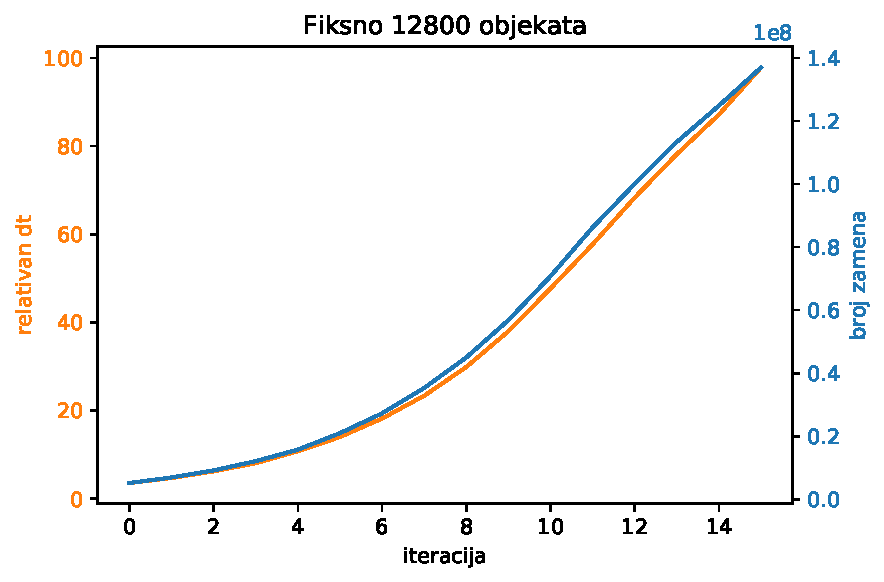
\includegraphics[
		trim=0 0 0 19,clip,
		scale=1]{dtSapCrawl.pdf}
	\caption{SAP: povratna sprega povećava $dt$, iako je fiksan broj objekata.}
	\label{fig:dtSapCrawl}
\end{figure}

Dok povećanje brzine kretanja može imati jako negativne posledice na performanse SAP algoritma,
smanjenje brzine kretanja utiče povoljno na njegovo vreme izvršavanja.
Poređenje vremena izvršavanja za tri različite brzine objekata je dato na slici \ref{fig:sap3speeds}. 
Podrazumevanja brzina objekata je $w/5$ jedinica u sekundi, gde je $w$ širina kontejnera unutar koga se objekti kreću.
Prvo merenje je izvršeno pri podrazumevanoj brzini, drugo pri duplo manjoj i treće pri četiri puta manjoj brzini.
Što se sporije objekti kreću to je tačka kada povratna sprega počinje da uzima maha više odložena.
Međutim, izvesno je da će se to u nekom trenutku desiti, tako da u zavisnosti od situacije SAP algoritam može biti loš ili idealan.

\begin{figure}[h!]
	\centerfloat
	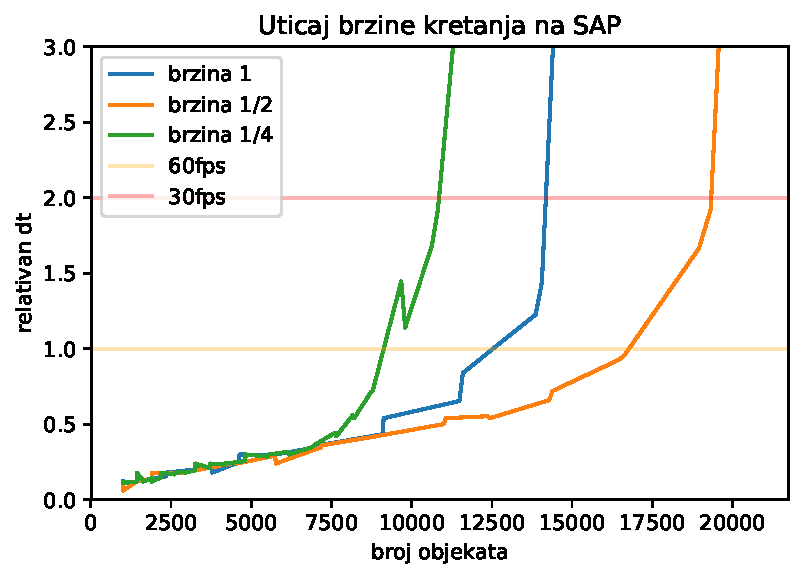
\includegraphics[
		trim=0 0 0 19,clip,
		scale=1]{sap3speeds.pdf}
	\caption{Upoređivanje rasta relativnog $dt$ u zavisnosti od broja objekata pri njihovim različitim brzinama - SAP.}
	\label{fig:sap3speeds}
\end{figure}

Svi do sada razmatrani algoritmi detekcije kolizije pre 20 000 objekata prelaze granicu od dva relativna $dt$.
Na slici \ref{fig:sap_great} je prikazan rezultat merenja gde se objekti kreću brzinom 64 puta sporijom od podrazumevane i tada je SAP algoritam ubedljivo najbolji.
Prilikom merenja je isključeno iscrtavanje pošto u ovom slučaju ono traje duže od samog algoritma detekcije kolizije,
što se može videti na slici \ref{fig:drawVsNoDraw}, gde tek za vrednosti bliske 50 000 objekata relativan $dt$ prelazi 2. 
Ovde je SAP višestruko bolji od ostalih, dostižući 60fps tek za 75 000, a 30fps za 92 000 objekata.
Pritom vrednost relativnog $dt$ ostaje ispod referentne prave koja označava linearnu zavisnost, sve do momenta kada se približava broju objekata koji dovodi 
do akumuliranja usporavanja, koji iznosi oko 100 000.


\begin{figure}[h!]
	\centerfloat
	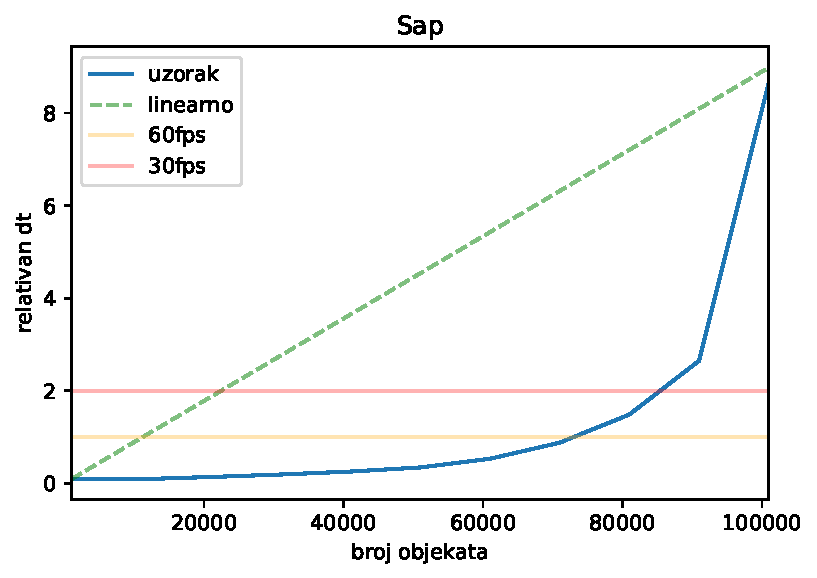
\includegraphics[
		trim=0 0 0 19,clip,
		scale=1]{sap_great.pdf}
	\caption{Relativan $dt$ u zavisnosti od broja objekata kada se objekti sporo kreću (64 puta sporije od podrazumevane brzine) - SAP.}
	\label{fig:sap_great}
\end{figure}

\section{Odabir algoritma detekcije kolizije}

Na osnovu grafika prikazanih u ovoj glavi se može primetiti da za drugačije
pozicije, brzine, veličine i brojeve objekata različiti algoritmi detekcije kolizije bivaju najefikasniji.
Može se zaključiti i da primenu trivijalnog algoritma, čije performanse su prikazane na slici \ref{fig:basic}, treba izbegavati.
Njega jedino ima smisla koristiti u slučaju kada je broj objekata manji od 100,
uz opravdanje da je jednostavan za implementaciju i lakše održiv zbog manje koda.
Međutim, uglavnom je potrebno imati algoritam detekcije kolizije koji će biti primenljiv i na više hiljada objekata,
tako da trivijalni algoritam ne dolazi u obzir.

U najvećem broju slučajeva oktri i njegove varijacije predstavljaju najbolji izbor.
Na osnovu rezultata prikazanih na grafiku \ref{fig:octree_leaf} preporuka je koristiti oktri sa maksimalnim brojem elemenata u listu 
postavljenim na 32, a dobar izbor maksimalne dubine je 10. 
Oktri sa duplikatima je bolji izbor u odnosu na oktri bez duplikata, osim ako može doći do stvaranja klastera objekata, kada
(prema grafiku \ref{fig:dupvsnodup}) oktri bez duplikata ima višestruko bolje performanse.

SAP algoritam je u opštem slučaju sporiji od oktrija i ne treba ga koristiti ako se većina objekata 
brzo kreće.
Ipak, SAP algoritam predstavlja najbolji izbor ako se skoro svi objekti kreću dovoljno malom brzinom 
tako da im je potrebno barem 100 sekundi da pređu širinu kontejnera u kome se nalaze.


% ==============================================================================
\chapter{Zaključak}
\label{sec:zakljucak}
% ==============================================================================

Virtuelni svetovi postaju grafički sve složeniji i interakcija sa njima verodostojnije oponaša fiziku pravog sveta.
Da bi takav nivo kompleksnosti bio moguć potrebno je koristiti bolji hardver, ali i bolji softver. 
Problem otkrivanja kolizija može postati usko grlo sistema i zato je potrebno pažljivo konstruisati 
algoritme i strukture podataka za njegovo efikasno rešavanje.

U tezi je dat pregled bitnih pojmova i fenomena koji utiču na detekciju kolizije, 
od kojih su najznačajniji vremenska koherentnost i konzistentnost vremena izvršavanja.
Opisani su algoritmi detekcije kolizije u realnom vremenu: osnovni algoritam, oktri sa duplikatima, oktri bez duplikata,
algoritam briši i odseci, i algoritam koji koristi ćelije i portale. 
Urađena je evaluacija ovih algoritama i izvršeno poređenje njihove efikasnosti.
Ispostavlja se da je u većini slučajeva najbolje koristiti oktri sa duplikatima.
Prepoznati su i formulisani i uslovi kada neki drugi algoritam predstavlja bolji izbor.

Kao glavni doprinos teze, implementiran je računarski program koji u realnom vremenu realizuje različite algoritme
za detekciju kolizije.
Program omogućava jednostavno podešavanje parametara algoritama i objekata čiji preseci se ispituju,
sa ciljem poređenja i odabira najboljeg algoritma u određenom slučaju.

Sledeći koraci za razvoj projekta bili bi usmereni ka istraživanju modifikacija oktrija 
i sličnih metoda particionisanja prostora.
U planu je i implementacija programa kojim bi se tokom izvršavanja programa dinamički birao najpogodniji algoritam iz skupa raspoloživih algoritama.
Na taj način bi se mogli izbeći najgori slučajevi za neke algoritme privremenim korišćenjem drugih  
algoritama otkrivanja kolizije.



% ------------------------------------------------------------------------------
% Literatura
% ------------------------------------------------------------------------------
\literatura

% ==============================================================================
% Završni deo teze i prilozi
\backmatter
% ==============================================================================


% \appendix
% \section{Dodatak}
% Dodatak.

\end{document}
